\documentclass[10pt]{beamer}
\usepackage[utf8]{inputenc}
\usepackage{xeCJK}
\usepackage{graphicx}
\usepackage {mathtools}
\usepackage{utopia} %font utopia imported
\usetheme{CambridgeUS}
\usecolortheme{dolphin}
\usepackage{pifont}

% set colors
\definecolor{myNewColorA}{RGB}{25,25,112}
\definecolor{myNewColorB}{RGB}{25,25,112}
\definecolor{myNewColorC}{RGB}{25,25,112}
\setbeamercolor*{palette primary}{bg=myNewColorC}
\setbeamercolor*{palette secondary}{bg=myNewColorB, fg = white}
\setbeamercolor*{palette tertiary}{bg=myNewColorA, fg = white}
\setbeamercolor*{titlelike}{fg=myNewColorA}
\setbeamercolor*{title}{bg=myNewColorA, fg = white}
\setbeamercolor*{item}{fg=myNewColorA}
\setbeamercolor*{caption name}{fg=myNewColorA}
\usefonttheme{professionalfonts}
\usepackage{natbib}
\usepackage{hyperref}
\usepackage{tikz}
%------------------------------------------------------------

\titlegraphic{
\includegraphics[height=1.5cm]{logo.jpg}} 

\setbeamerfont{title}{size=\large}
\setbeamerfont{subtitle}{size=\small}
\setbeamerfont{author}{size=\small}
\setbeamerfont{date}{size=\small}
\setbeamerfont{institute}{size=\small}

\title[Explicații]{\textbf{Fenomenele fizice din spatele aplicațiilor G4}}

%\subtitle{ }
\author[Andreicovici Iulian Florin]{\textbf{Andreicovici Iulian Florin}}

\institute[UPB]{\textit{Universitatea Politehnica din București - UPB}}

\date[\textcolor{white}{\today} ]
{\today}

%------------------------------------------------------------
%This block of commands puts the table of contents at the 
%beginning of each section and highlights the current section:
%\AtBeginSection[]
%{
%  \begin{frame}
%    \frametitle{Contents}
%    \tableofcontents[currentsection]
%  \end{frame}
%}
\AtBeginSection[]{
  \begin{frame}
  \vfill
  \centering
  \begin{beamercolorbox}[sep=8pt,center,shadow=true,rounded=true]{title}
    \usebeamerfont{title}\insertsectionhead\par%
  \end{beamercolorbox}
  \vfill
  \end{frame}
}
%------------------------------------------------------------

\begin{document}

%The next statement creates the title page.
\frame{\titlepage}
\begin{frame}
\frametitle{Contents}
\tableofcontents
\end{frame}
%------------------------------------------------------------

%dușul atmosferic - sect 1
\section{\textbf{ Jetul atmosferic - ce este și cum se produce}}
  
  
  \begin{frame}{\textbf{Despre Jetul atmosferic}}
 \vspace{-1cm}

  \begin{itemize}
    
      \item[\ding{51}] \makebox[0.5cm]{} \textbf{ Este o "rețea în cascadă" de particule ionizate și radiație electromagnetică care se formează atunci când radiația cosmică pătrunde în atmosferă și interacționează cu moleculele gazelor atmosferice.} \\
      
      \item[\ding{51}] \makebox[0.5cm]{} \textbf{ Desemnează un jet de numeroase particule, multe de natură hadronică - în special sub formă de pioni, kaoni și barioni care se formează la interacția dintre o moleculă sau un atom din atmosferă cu o particulă incidentă.}\\
     
     \item[\ding{51}] \makebox[0.5cm]{} \textbf{ Particula incidentă poate fi: $p^+$, $n^0$, $e^-$, un nucleu, o rază gamma sau chiar un $e^+$.}

     \item[\ding{51}] \makebox[0.5cm]{} \textbf{ Particulele secundare pot interacționa la rândul lor cu alte particule, formând o cascadă "în lanț" de produse secundare care sunt expulzate în mai toate direcțiile.}
   
  \end{itemize}
 
    \end{frame}


%frame2
\begin{frame}{\textbf{Cum arată jetul atmosferic}}
  
\begin{tikzpicture}[overlay, remember picture]
\node[anchor=center, 
      xshift=0cm, 
      yshift=-0.5cm] 
     at (current page.center) 
     {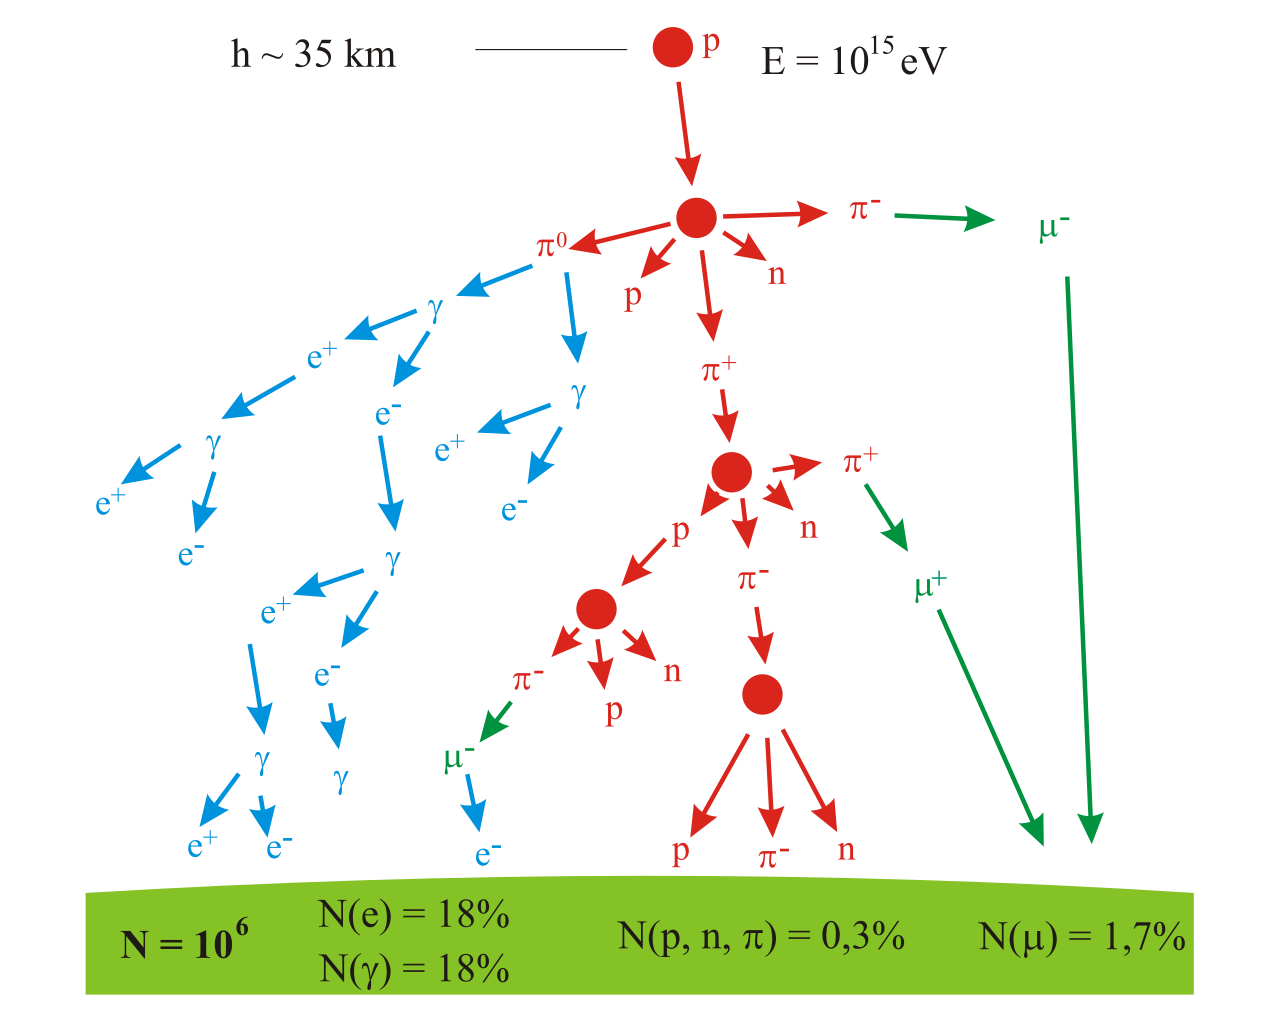
\includegraphics[scale=0.2]{Imagini/1280px-AirShower.png}};
\end{tikzpicture}
 \end{frame}


%frame3
\begin{frame}{\textbf{\underline{Ce fel de particule conține}}}
  
\begin{tikzpicture}[overlay, remember picture]
\node[anchor=center, 
      xshift=0cm, 
      yshift=-0.5cm] 
     at (current page.center) 
     {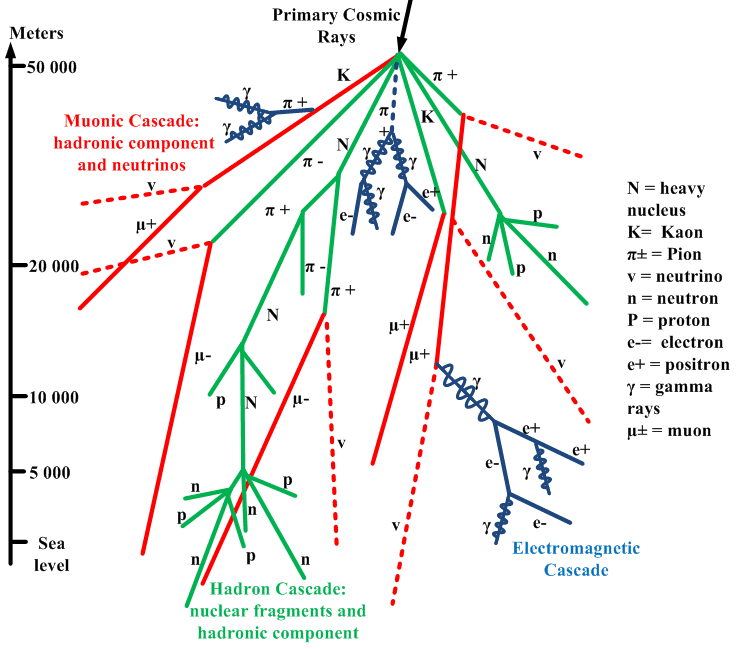
\includegraphics[scale=0.3]{Imagini/Showers-of-cosmic-ray-reactions-with-particles-of-the-atmosphere-Clo02-1.png}};
\end{tikzpicture}
 \end{frame}


%frame4
\begin{frame}{\textbf{Jetul atmosferic generate un proton relativist}}
  
\begin{tikzpicture}[overlay, remember picture]
\node[anchor=center, 
      xshift=0cm, 
      yshift=-0.5cm] 
     at (current page.center) 
     {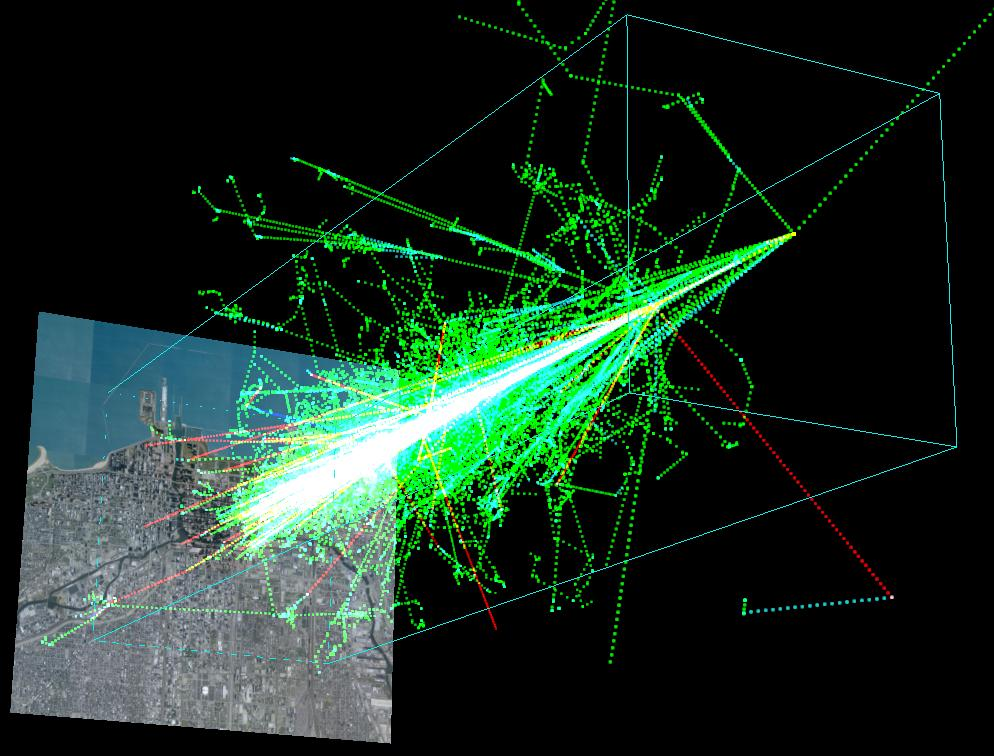
\includegraphics[scale=0.27]{Imagini/Protonshower.jpg}};
\end{tikzpicture}

 \end{frame}


%frame5
\begin{frame}{\textbf{\underline{Detalii relevante}}}
  
\vspace{-2.5cm}

  \begin{itemize}
    \small
      \item[\ding{55}] \textbf{ Diverse interacțiuni hadronice au loc iar în baia de particule rezultate mare parte au tendința de a se mișca pe aceeași direcție cu particula primară.} \\
      
      \item[\ding{55}] \textbf{ Produsele secundare formează ramurile unui mănunchi ramificat și interacționează cu alte molecule de gaze, generând excitarea acestora.}\\
     
     \item[\ding{55}] \textbf{ Diverse canale de dezintegrare sunt reperate prin detectarea la sol a radiațiilor rezultate.}

     \item[\ding{55}] \textbf{ Particulele secundare pot interacționa la rândul lor cu alte particule, inducând un jet de alte produse.}
   
  \end{itemize}
 
 \begin{tikzpicture}[overlay, remember picture]
\node[anchor=center, 
      xshift=-2cm, 
      yshift=-2cm] 
     at (current page.center) 
     {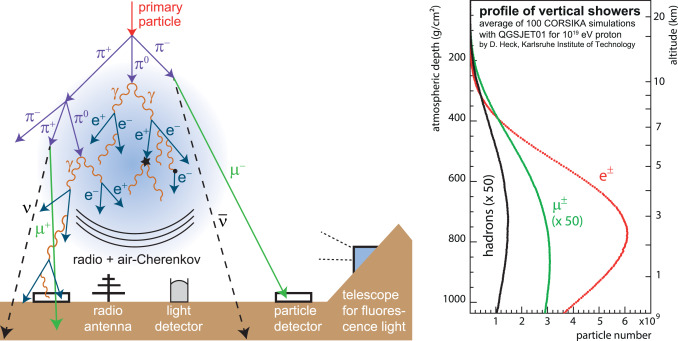
\includegraphics[scale=0.4]{Imagini/Im.png}};
\end{tikzpicture}

 \begin{tikzpicture}[overlay, remember picture]
\node[anchor=center, 
      xshift= 3.5cm, 
      yshift=-2cm] 
     at (current page.center) 
     {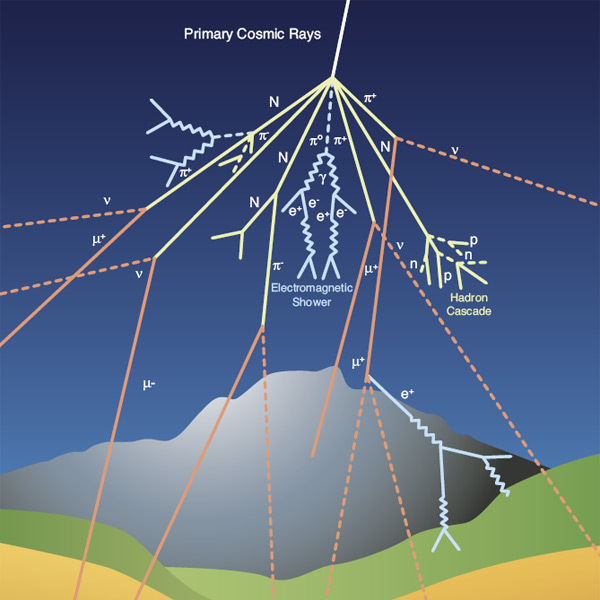
\includegraphics[scale=0.22]{Imagini/cosmic_ray.jpg}};
\end{tikzpicture}

\end{frame}


%frame5
\begin{frame}{\textbf{Numeroase canale de dezintegrare}}

 \begin{tikzpicture}[overlay, remember picture]
\node[anchor=center, 
      xshift=0cm, 
      yshift=0cm] 
     at (current page.center) 
     {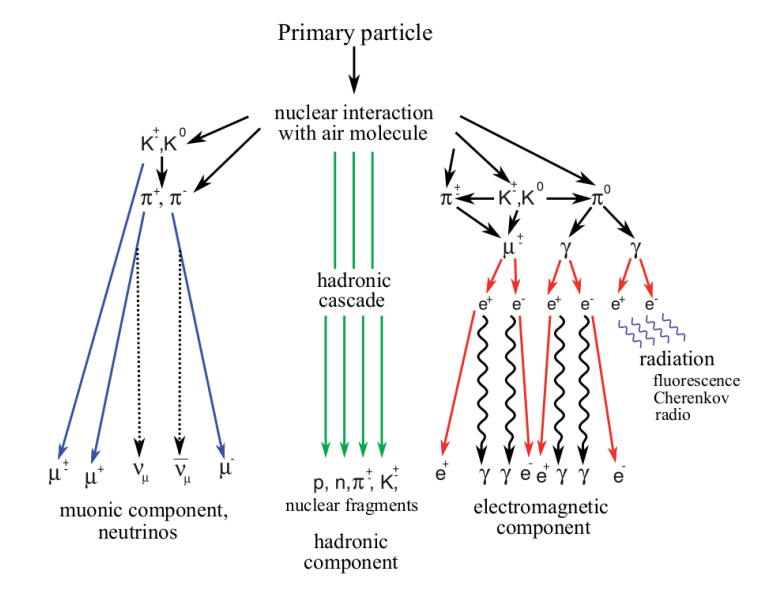
\includegraphics[scale=0.45]{Imagini/MyShower.png}};
\end{tikzpicture}

 \end{frame}


%frame6
\begin{frame}

 \begin{tikzpicture}[overlay, remember picture]
\node[anchor=center, 
      xshift=0cm, 
      yshift=0cm] 
     at (current page.center) 
     {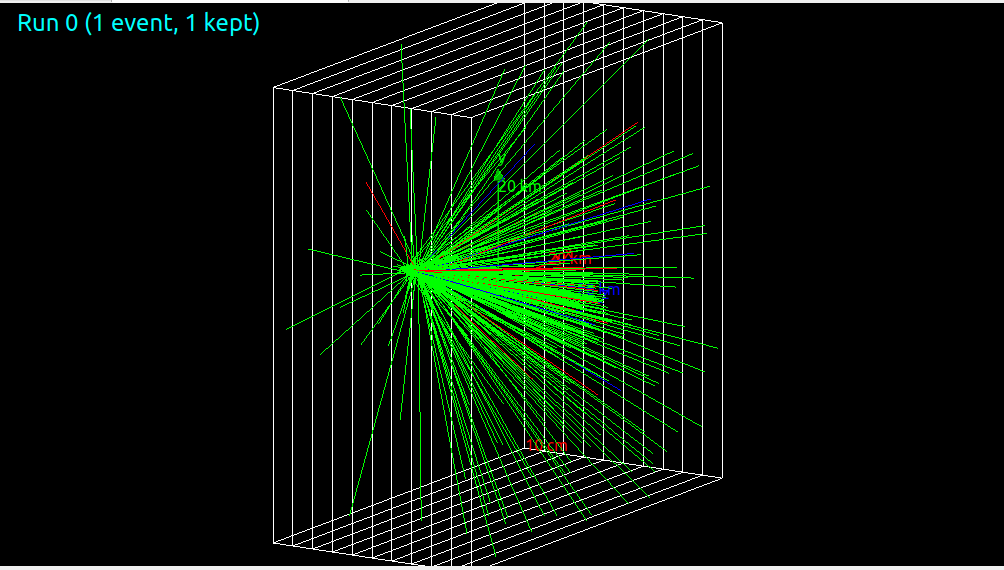
\includegraphics[scale=0.45]{Imagini/DusulMeu.png}};
\end{tikzpicture}

 \end{frame}


%frame7
\begin{frame}{\textbf{\underline{Simularea mea}}}

 \begin{tikzpicture}[overlay, remember picture]
\node[anchor=center, 
      xshift=-3.5cm, 
      yshift=1cm] 
     at (current page.center) 
     {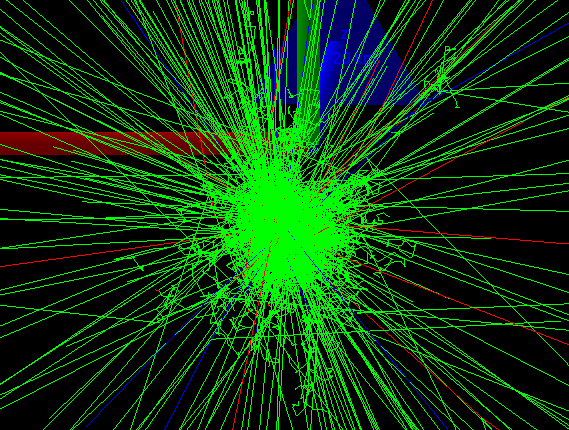
\includegraphics[scale=0.25]{Imagini/vertex.png}};
\end{tikzpicture}

 \begin{tikzpicture}[overlay, remember picture]
\node[anchor=center, 
      xshift=2.8cm, 
      yshift=1cm] 
     at (current page.center) 
     {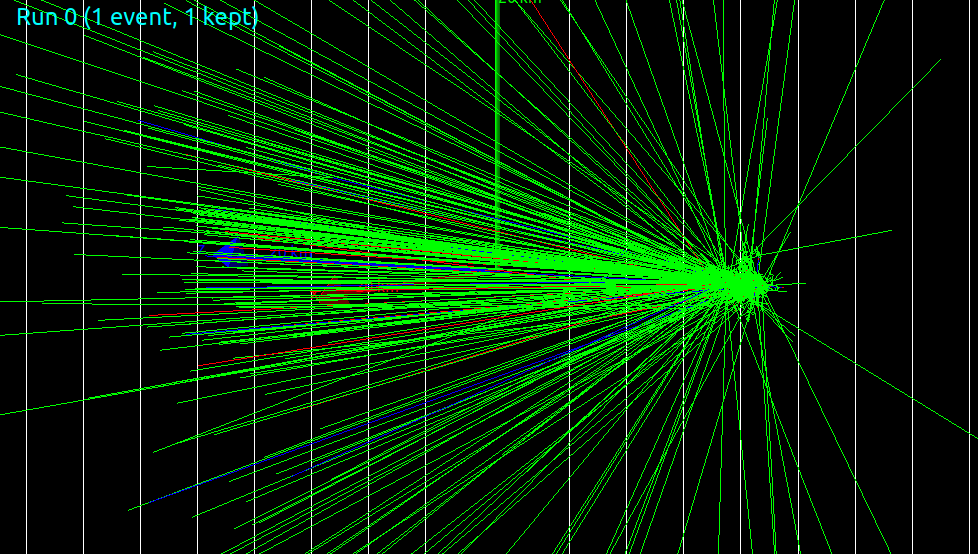
\includegraphics[scale=0.2]{Imagini/vertexuri.png}};
\end{tikzpicture}

\vspace{3.7cm}

\begin{itemize}
 

     \item[\ding{35}] \makebox[0.5cm]{} \textit {\textbf{ Simularea grafică a jetului de particule care rezultă din interacțiunea unui proton cu Ec = 100 GeV și 10 straturi de atmosferă. Multiple ramificații sunt alocate unor radiații gamma rezultate din dezintegrarea pionilor(tracks-urile verzi).}}

\end{itemize}
 \end{frame}




%secțiunea 2 - detectorul HPGe
\section{\textbf{ Cum funcționează detectorul cu germaniu hiperpur?}}

%frame8
\begin{frame}{\textbf{Detectorul HPGe - principii}}

\begin{itemize}

\vspace{-0.5cm}
\item[\ding{45}] \textbf{- Reprezintă un detector cu semiconductor(Ge) ca zonă activă și are o bună rezoluție energetică - motiv pentru care este folosit în spectrometria gamma.}\\
\item[\ding{45}] \textbf{- Ge are o energie mai mică(față de Si) necesară formării unei perechi electron-gol cât și o probabilitate mai mare de interacție cu radiația gamma(deoarece posedă un număr de masă mai mare.)}\\
\item[\ding{45}] \textbf{- Radiația gamma are o energie suficientă pentru a ioniza atomii de Germaniu; pe măsură ce pătrunde în stratul de material va genera numeroase perechi electron-gol.}\\
\item[\ding{45}] \textbf{- Sub influența unui câmp electric exterior, atât golurile cât și electronii se vor deplasa spre electrozi de unde se poate obține un impuls electric măsurabil printr-un circuit exterior.}
\\---------------------------------------------------------------------------------------------   
\end{itemize}

\end{frame}


%frame9
\begin{frame}{\textbf{\underline{Schema detectorului}}}

 \begin{tikzpicture}[overlay, remember picture]
\node[anchor=center, 
      xshift=-3cm, 
      yshift=1cm] 
     at (current page.center) 
     {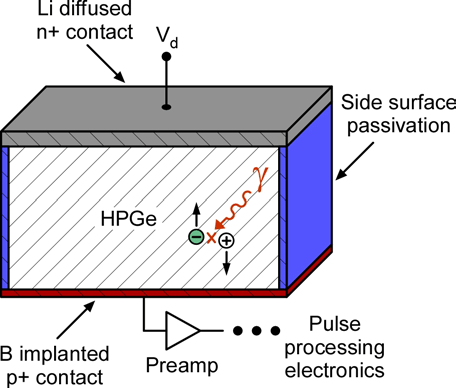
\includegraphics[scale=0.3]{Imagini/Schematic-cross-sectional-drawings-of-HPGe-based-radiation-detectors-constructed-using.png}};
\end{tikzpicture}

 \begin{tikzpicture}[overlay, remember picture]
\node[anchor=center, 
      xshift=2.6cm, 
      yshift=1cm] 
     at (current page.center) 
     {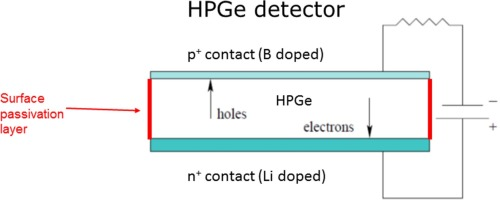
\includegraphics[scale=0.55]{Imagini/all.png}};
\end{tikzpicture}

\vspace{4cm}

\begin{itemize}
   
\small
 \item[!] \makebox[0.5cm]{} \textbf{ Zona din germaniu activ este căptușită la interior cu un strat din Bor și la exterior cu unul din Litiu - se formează o joncțiune p-n iar electronii odată trecuți în banda de conducție vor fi dirijați spre zona din litiu(zona n) și golurile spre zona p(din B) - polaritate inversă.} 
\end{itemize}

\end{frame}


%frame 10
\begin{frame}{\textbf{Părțile unui detector HPGe}}
 \begin{tikzpicture}[overlay, remember picture]
\node[anchor=center, 
      xshift=0cm, 
      yshift=0cm] 
     at (current page.center) 
     {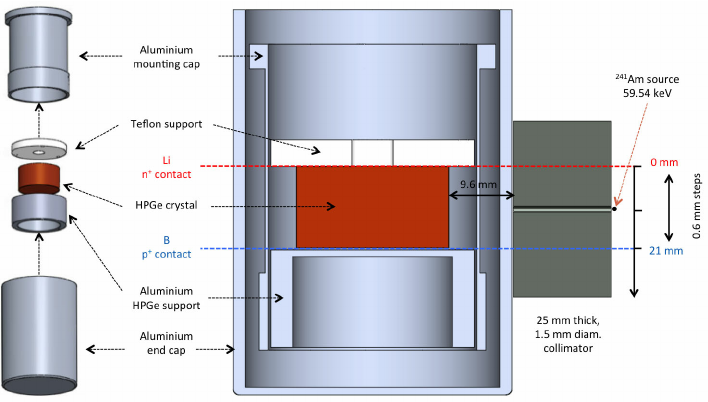
\includegraphics[scale=0.4]{Imagini/Left-Layout-scheme-of-the-cryostat-and-supports-of-the-HPGe-crystal-Right-Cross.png}};
\end{tikzpicture}
\end{frame}


%frame 11
\begin{frame}{\textbf{Geometria detectorului meu HPGe}}
 \begin{tikzpicture}[overlay, remember picture]
\node[anchor=center, 
      xshift=0cm, 
      yshift=0cm] 
     at (current page.center) 
     {
\includegraphics[scale=0.3]{Imagini/Detector.png}};
\end{tikzpicture}
\end{frame}


%frame 12
\begin{frame}{\textbf{Schița detectorului meu HPGe}}

 \begin{tikzpicture}[overlay, remember picture]
\node[anchor=center, 
      xshift=-3.5cm, 
      yshift=0.5cm] 
     at (current page.center) 
     {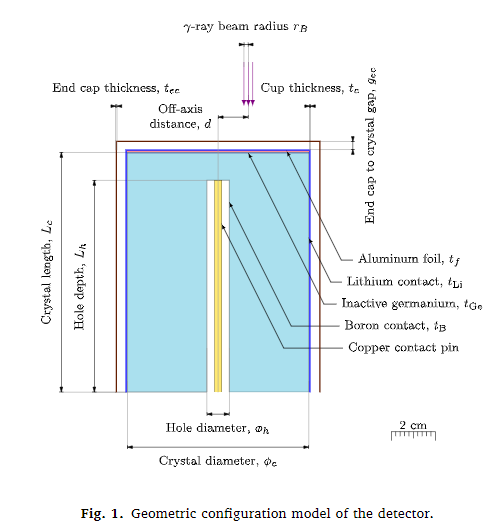
\includegraphics[scale=0.4]{Imagini/Configruation.png}};
\end{tikzpicture}

 \begin{tikzpicture}[overlay, remember picture]
\node[anchor=center, 
      xshift=2.9cm, 
      yshift=0cm] 
     at (current page.center) 
     {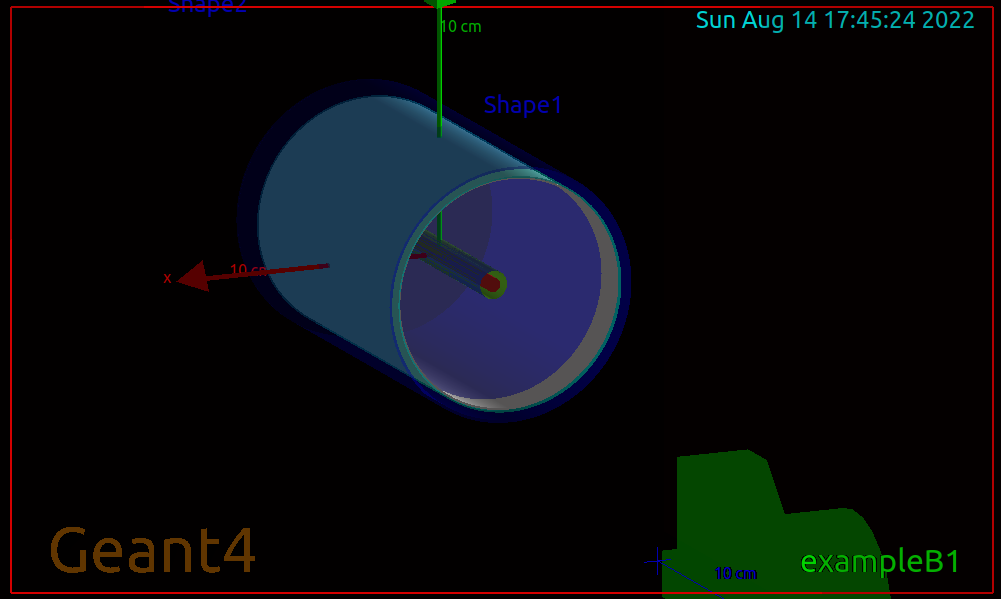
\includegraphics[scale=0.18]{Imagini/MicrosoftTeams-image.png}};
\end{tikzpicture}

\vspace{4.5cm}
\small

\begin{itemize}
    \item \makebox[0.5cm]{} \textit{\textbf{Numărul perechilor electron-gol formate prin ionizare este proporțional cu intensitatea radiației captate. Spre exemplu, o cuantă $\gamma$ cu E = 1 MeV va lăsa în urma sa cca. $10^5$ perechi electron-gol.}}
\end{itemize}

\begin{tikzpicture}[overlay, remember picture]
\node[anchor=center, 
      xshift=2.9cm, 
      yshift=0cm] 
     at (current page.center) 
     {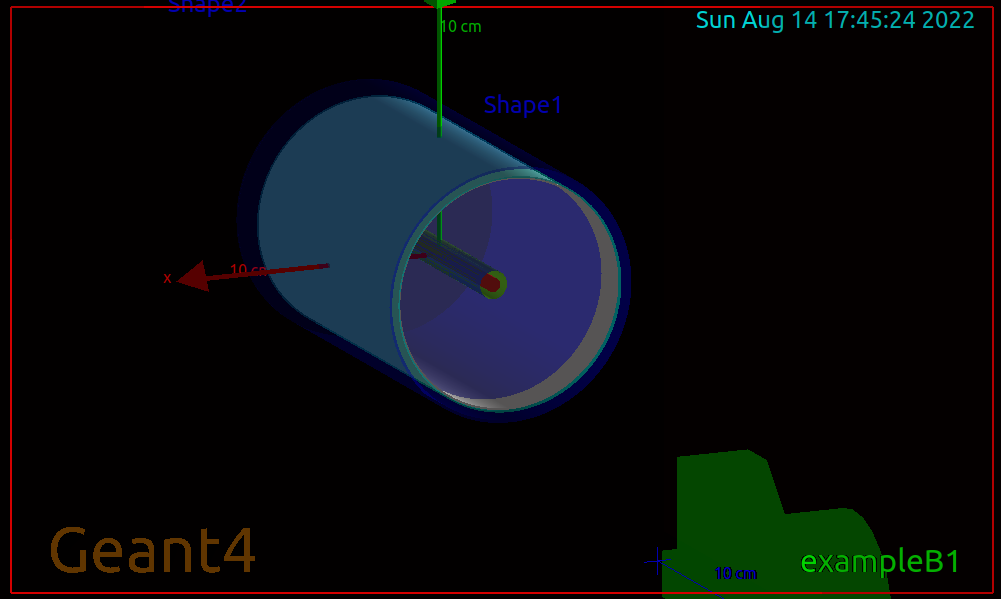
\includegraphics[scale=0.18]{Imagini/MicrosoftTeams-image.png}};
\end{tikzpicture}


\end{frame}


%frame 13
\begin{frame}{\textbf{\underline{Ce am obținut}}}

\begin{itemize}

\vspace{-3cm}
   \item  \textbf{Reprezentarea numărului de intrări(sau de fotonii detectați) în funcție de valorile lor energetice - spectrele surselor.}\\
   \item \textbf{Afișarea grafică a distribuției spațiale de fotoni/particule.}\\
   \item \textbf{Calculul depozitelor energetice care au fost stocate în zona activă din Ge.}

\end{itemize}

\begin{tikzpicture}[overlay, remember picture]
\node[anchor=center, 
      xshift=2.5cm, 
      yshift=-2cm] 
     at (current page.center) 
     {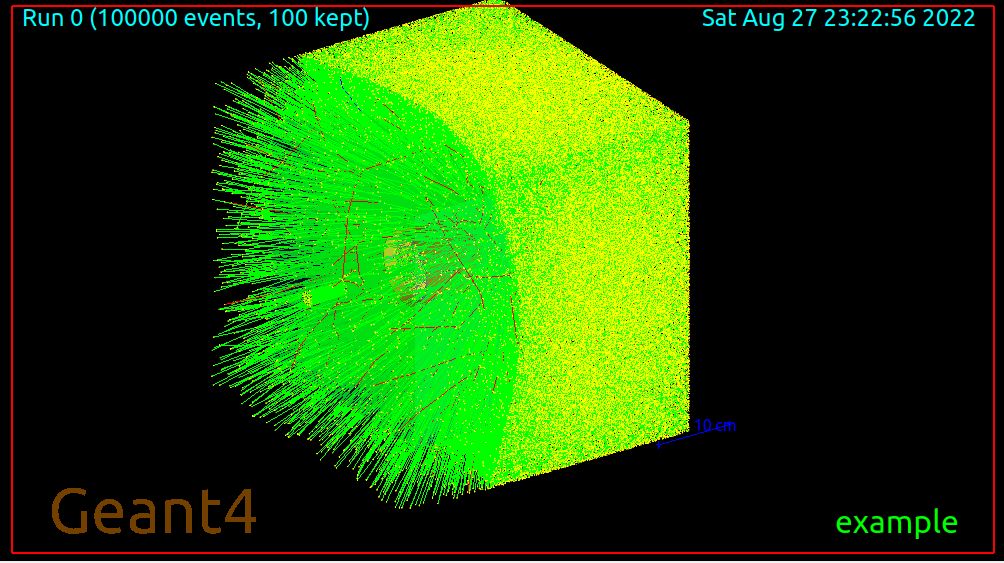
\includegraphics[scale=0.2]{Imagini/MST.png}};
\end{tikzpicture} 

\begin{tikzpicture}[overlay, remember picture]
\node[anchor=center, 
      xshift=-3.5cm, 
      yshift=-2cm] 
     at (current page.center) 
     {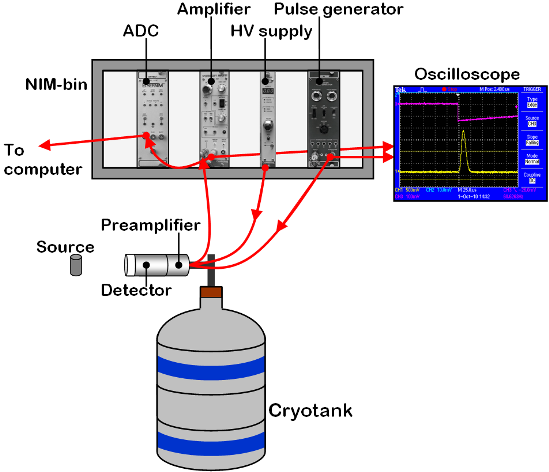
\includegraphics[scale=0.2]{Imagini/Gamma_spectroscopy_setup_schematics.png}};
\end{tikzpicture} 

\end{frame}


%frame14
\begin{frame}{\textbf{\underline{\small Na22 - Spectrul aferent procesării a 10.000 de evenimente}}}

\begin{tikzpicture}[overlay, remember picture]
\node[anchor=center, 
      xshift=0cm, 
      yshift=0cm] 
     at (current page.center) 
     {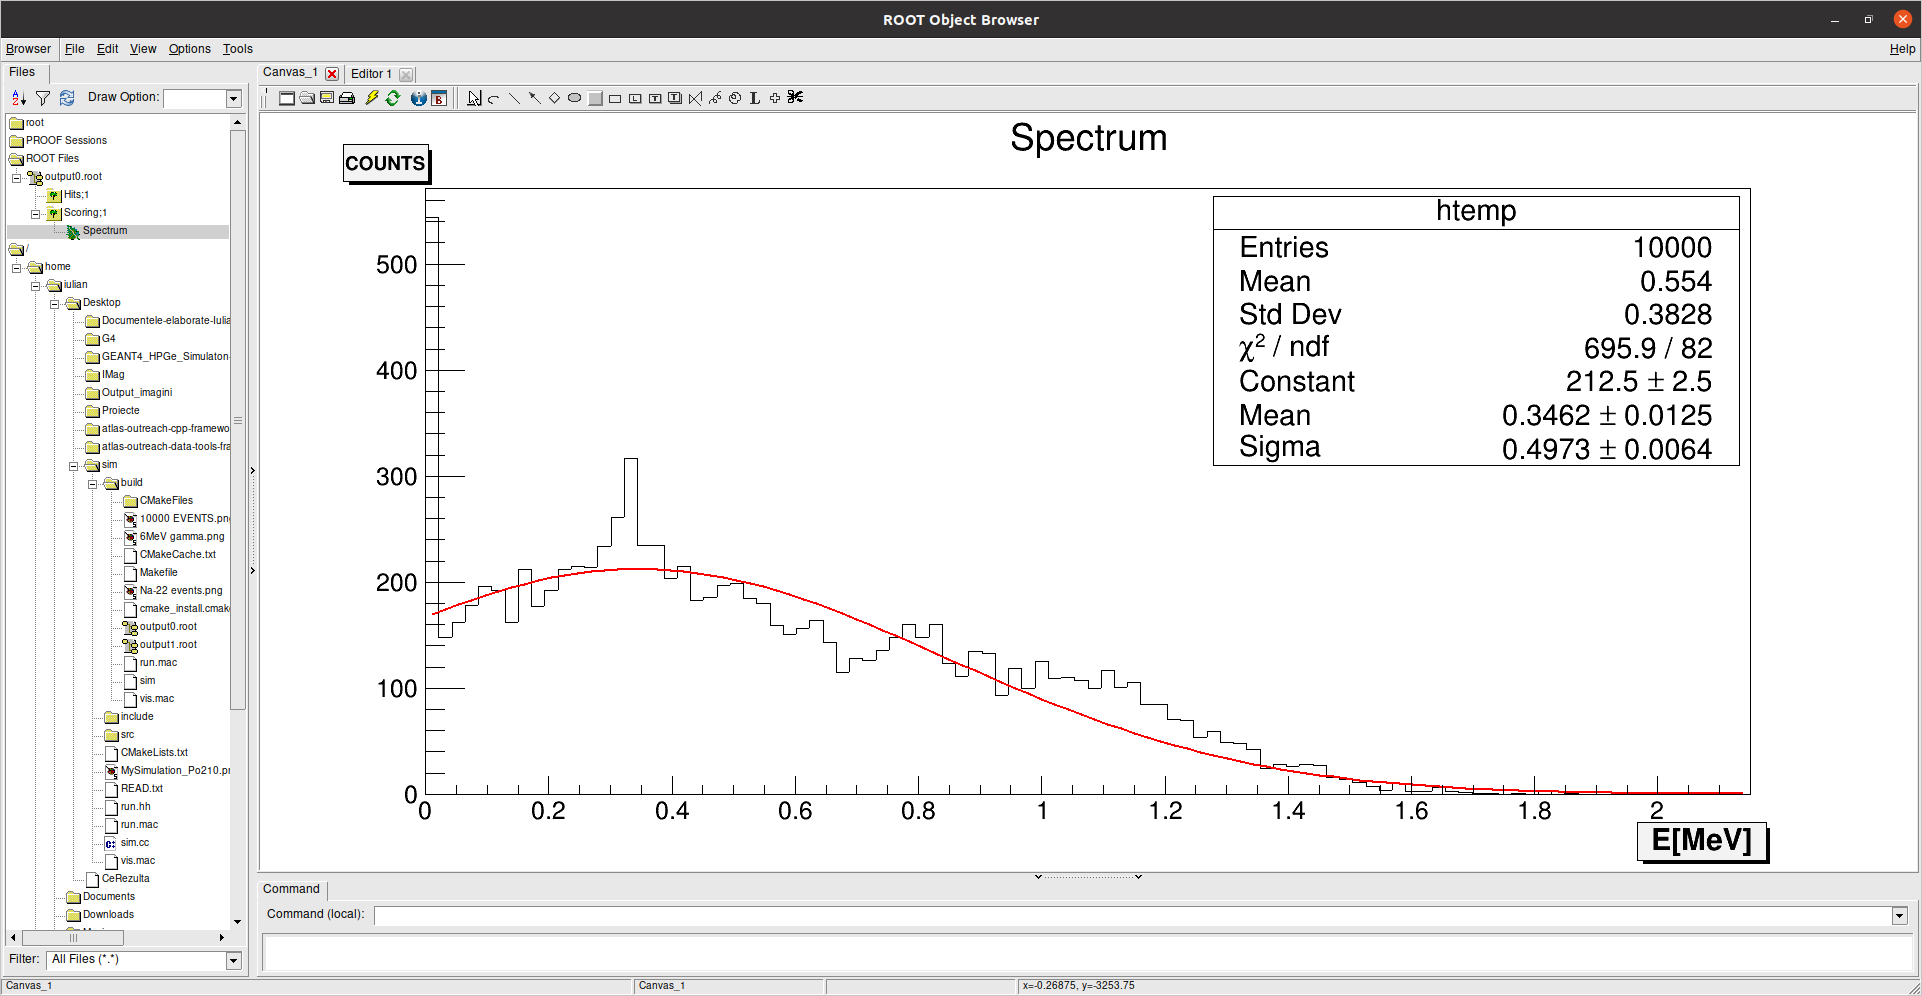
\includegraphics[scale=0.2]{Imagini/Screenshot from 2022-08-30 16-29-40.png}};
\end{tikzpicture} 

\end{frame}

%frame15
\begin{frame}{\textbf{\underline{Na22 display 10.000 Events}}}

\begin{tikzpicture}[overlay, remember picture]
\node[anchor=center, 
      xshift=0cm, 
      yshift=0cm] 
     at (current page.center) 
     {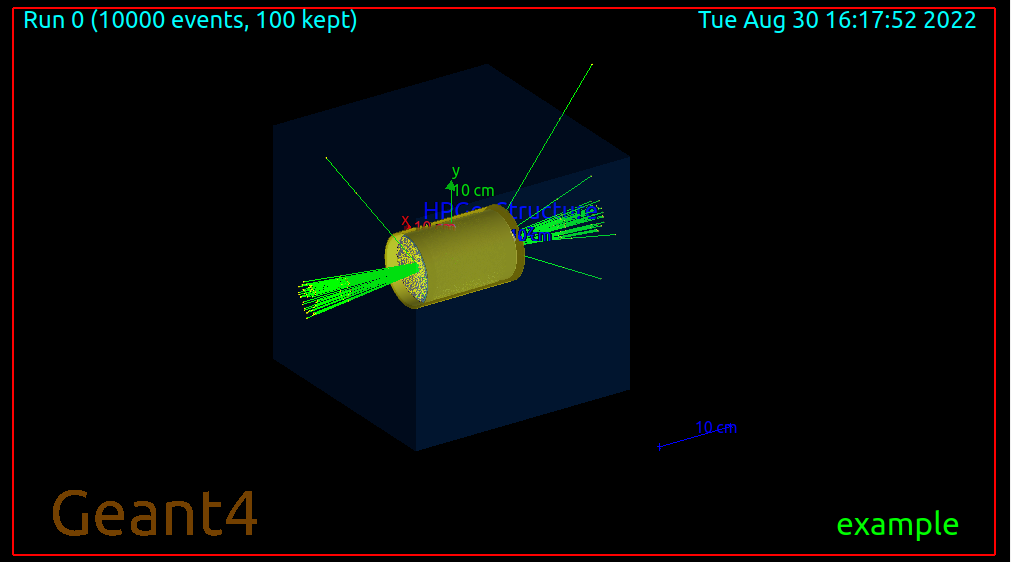
\includegraphics[scale=0.35]{Imagini/Screenshot from 2022-08-30 16-18-53.png}};
\end{tikzpicture} 

\end{frame}


\begin{frame}{\textbf{\underline{Na22 canal de dezintegrare}}}
\begin{tikzpicture}[overlay, remember picture]
\node[anchor=center, 
      xshift=0cm, 
      yshift=0cm] 
     at (current page.center) 
     {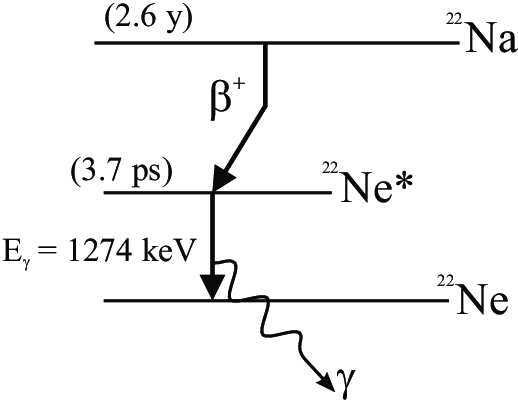
\includegraphics[scale=0.35]{Imagini/Ne.png}};
\end{tikzpicture} 


\end{frame}


%frame16
\begin{frame}{\textbf{\underline{\small Pa234 - Spectrul aferent procesării a 2.000 de evenimente}}}

\begin{tikzpicture}[overlay, remember picture]
\node[anchor=center, 
      xshift=0cm, 
      yshift=0cm] 
     at (current page.center) 
     {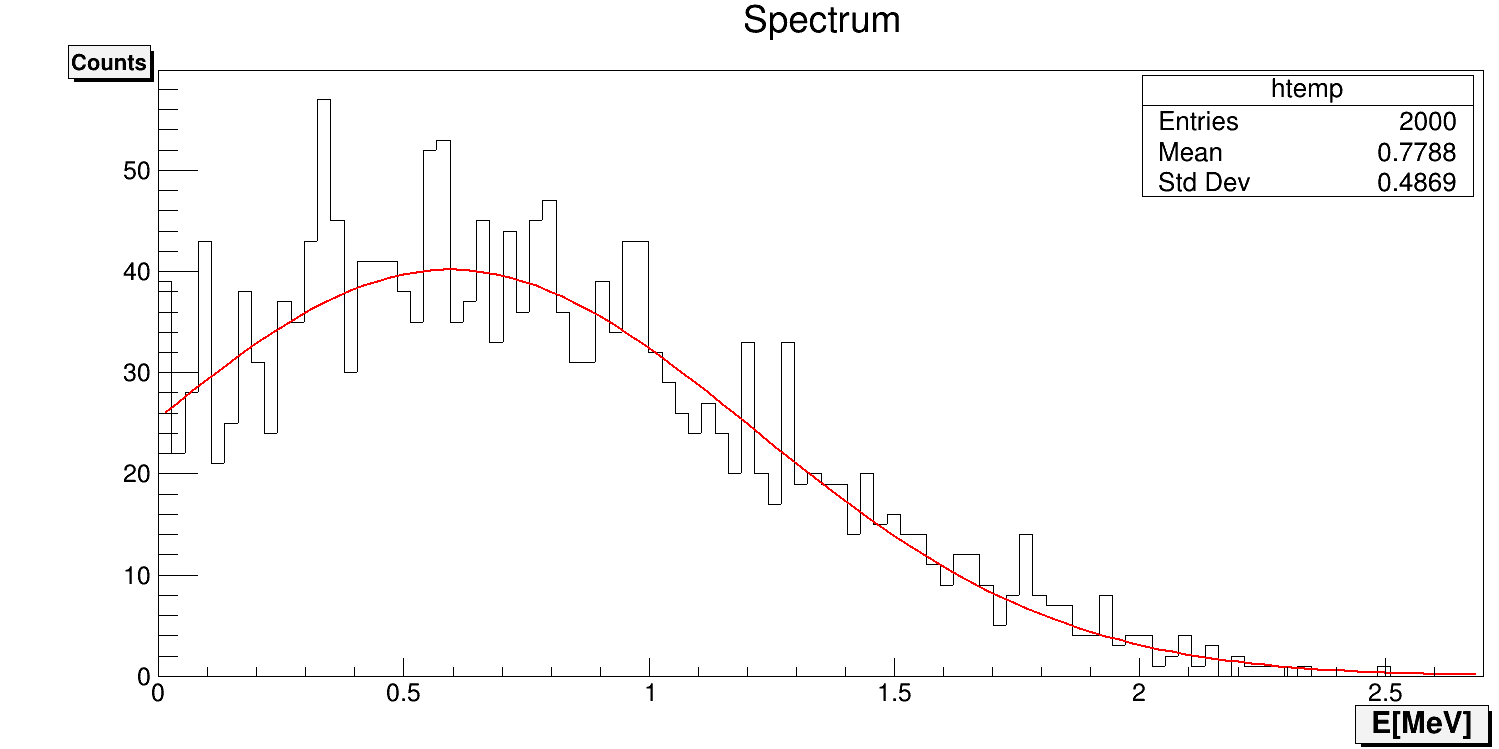
\includegraphics[scale=0.22]{Imagini/Pa234Spectrum.png}};
\end{tikzpicture} 

\end{frame}


\begin{frame}{\textbf{\underline{\small Pa234 - afișarea celor 2.000 de evenimente}}}

\begin{tikzpicture}[overlay, remember picture]
\node[anchor=center, 
      xshift=0cm, 
      yshift=0cm] 
     at (current page.center) 
     {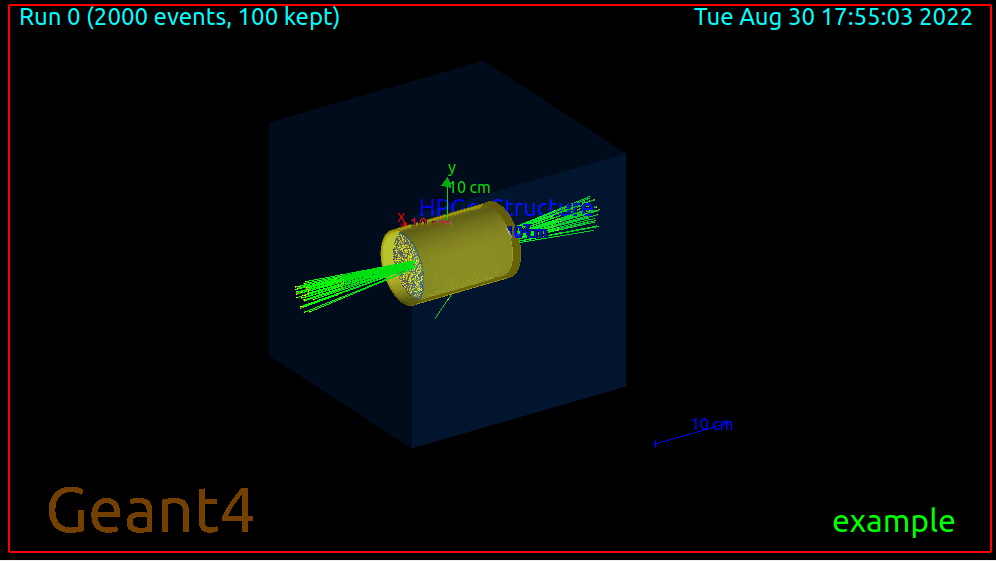
\includegraphics[scale=0.35]{Imagini/Pa234.png}};
\end{tikzpicture} 

\end{frame}

%frame17
\begin{frame}{\textbf{\underline{Eu152 - spectrul simulat}}}

\begin{tikzpicture}[overlay, remember picture]
\node[anchor=center, 
      xshift=0cm, 
      yshift=0cm] 
     at (current page.center) 
     {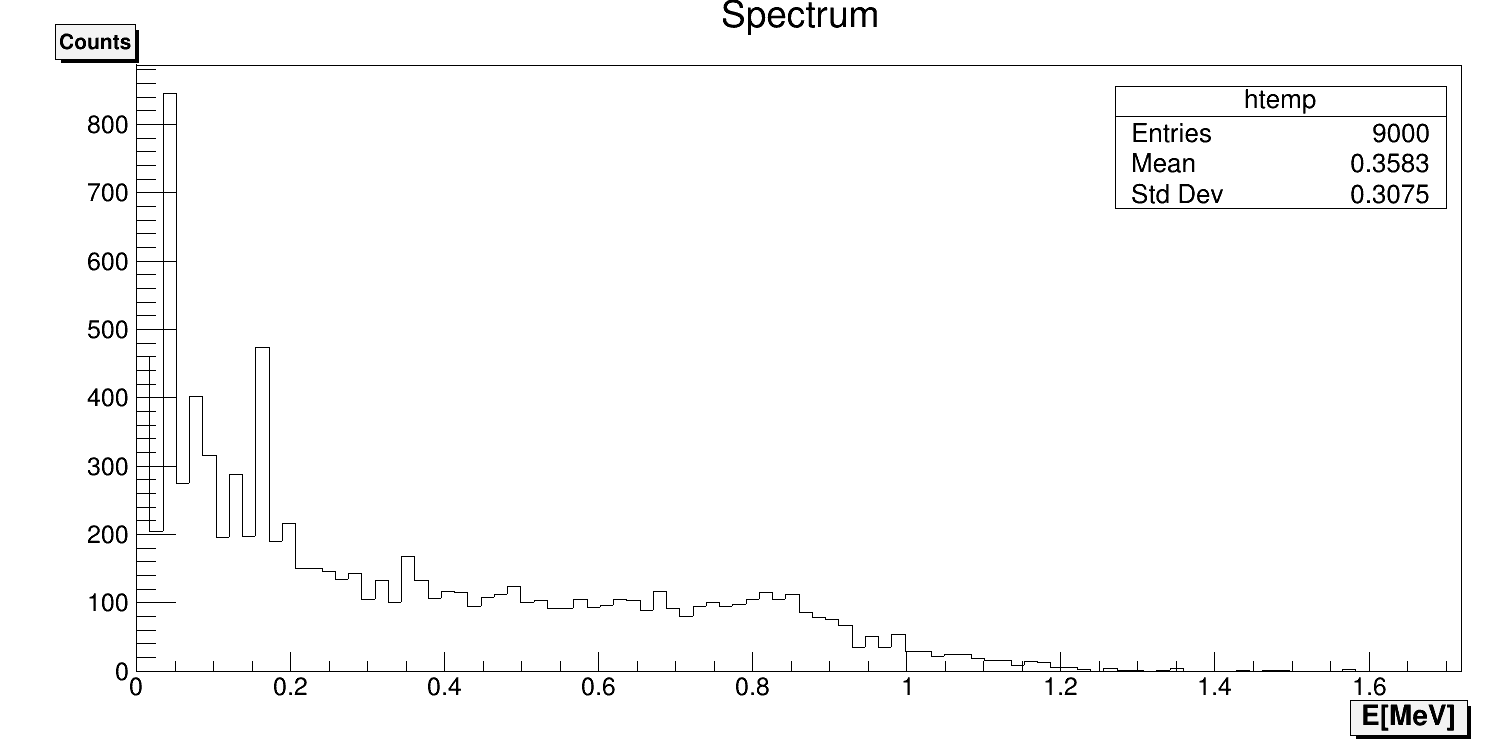
\includegraphics[scale=0.25]{Imagini/Eu-152(simulation).png}};
\end{tikzpicture} 

\end{frame}


% detectorul de radiatie Cherenkov - final
\section{\textbf{Detectorul de radiație Cherenkov}}
   
\begin{frame}{\textbf{\underline{Ce este radiația Cherenkov}}}
\begin{itemize}

\vspace{-3cm}
   \item \makebox[0.5cm]{} \textbf{Este radiația emisă ca urmare a depășirii vitezei de fază a luminii printr-un mediu de către o particulă materială cu sarcină electrică.}\\
   \item \makebox[0.5cm]{} \textbf{Particula incidentă deformează norii electronici ai atomilor și induce dipoli temporari - dezexcitarea acestor dipoli este însoțită de o emisie corentă de fotoni.}\\

\end{itemize}

\begin{tikzpicture}[overlay, remember picture]
\node[anchor=center, 
      xshift=-2cm, 
      yshift=-2cm] 
     at (current page.center) 
     {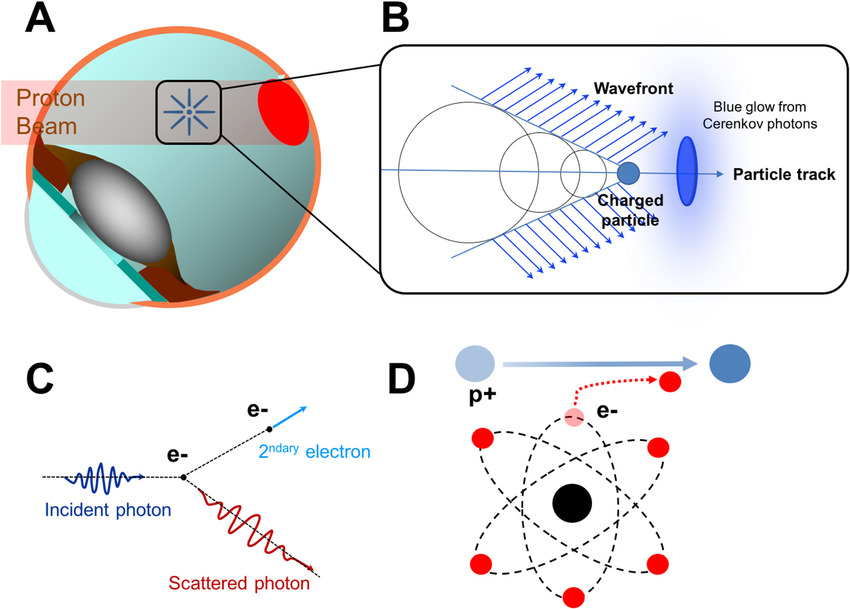
\includegraphics[scale=0.2]{Imagini/Role-of-the-Cherenkov-radiation-in-the-occurrence-of-phosphenes-in-patients-irradiated-by.jpg}};
\end{tikzpicture} 

\begin{tikzpicture}[overlay, remember picture]
\node[anchor=center, 
      xshift=3.5cm, 
      yshift=-2cm] 
     at (current page.center) 
     {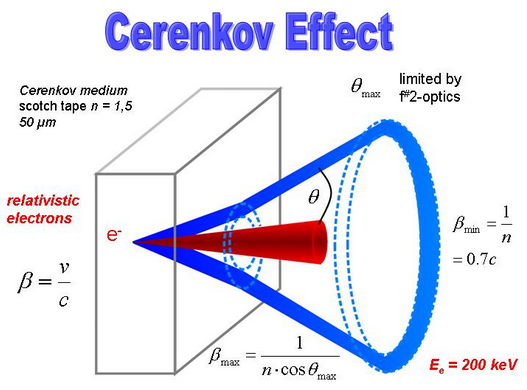
\includegraphics[scale=0.3]{Imagini/radiation-therapy.png}};
\end{tikzpicture} 

\end{frame}


%frame18

\begin{frame}{\textbf{\underline{\small Frontul radiației Cherenkov- unghiul Cherenkov}}}

\begin{tikzpicture}[overlay, remember picture]
\node[anchor=center, 
      xshift=-4cm, 
      yshift=0cm] 
     at (current page.center) 
     {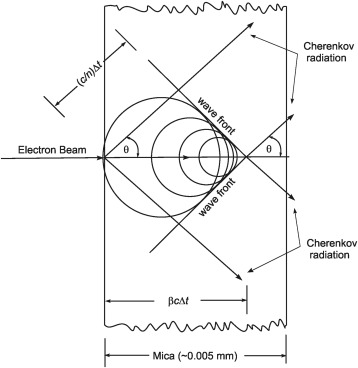
\includegraphics[scale=0.6]{Imagini/3-s2.0-B9780128143957000064-f06-06-9780128143957.jpg}};
\end{tikzpicture} 


\begin{tikzpicture}[overlay, remember picture]
\node[anchor=center, 
      xshift=-4cm, 
      yshift=-3cm] 
     at (current page.center) 
     {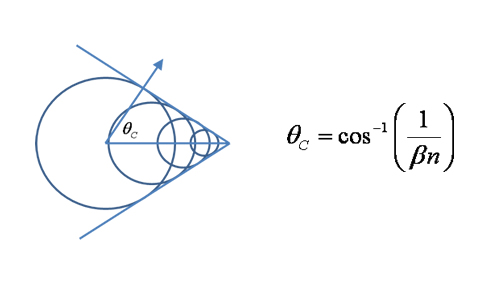
\includegraphics[scale=0.6]{Imagini/cherenkovring.jpg}};
\end{tikzpicture} 


\begin{tikzpicture}[overlay, remember picture]
\node[anchor=center, 
      xshift=3cm, 
      yshift=0cm] 
     at (current page.center) 
     {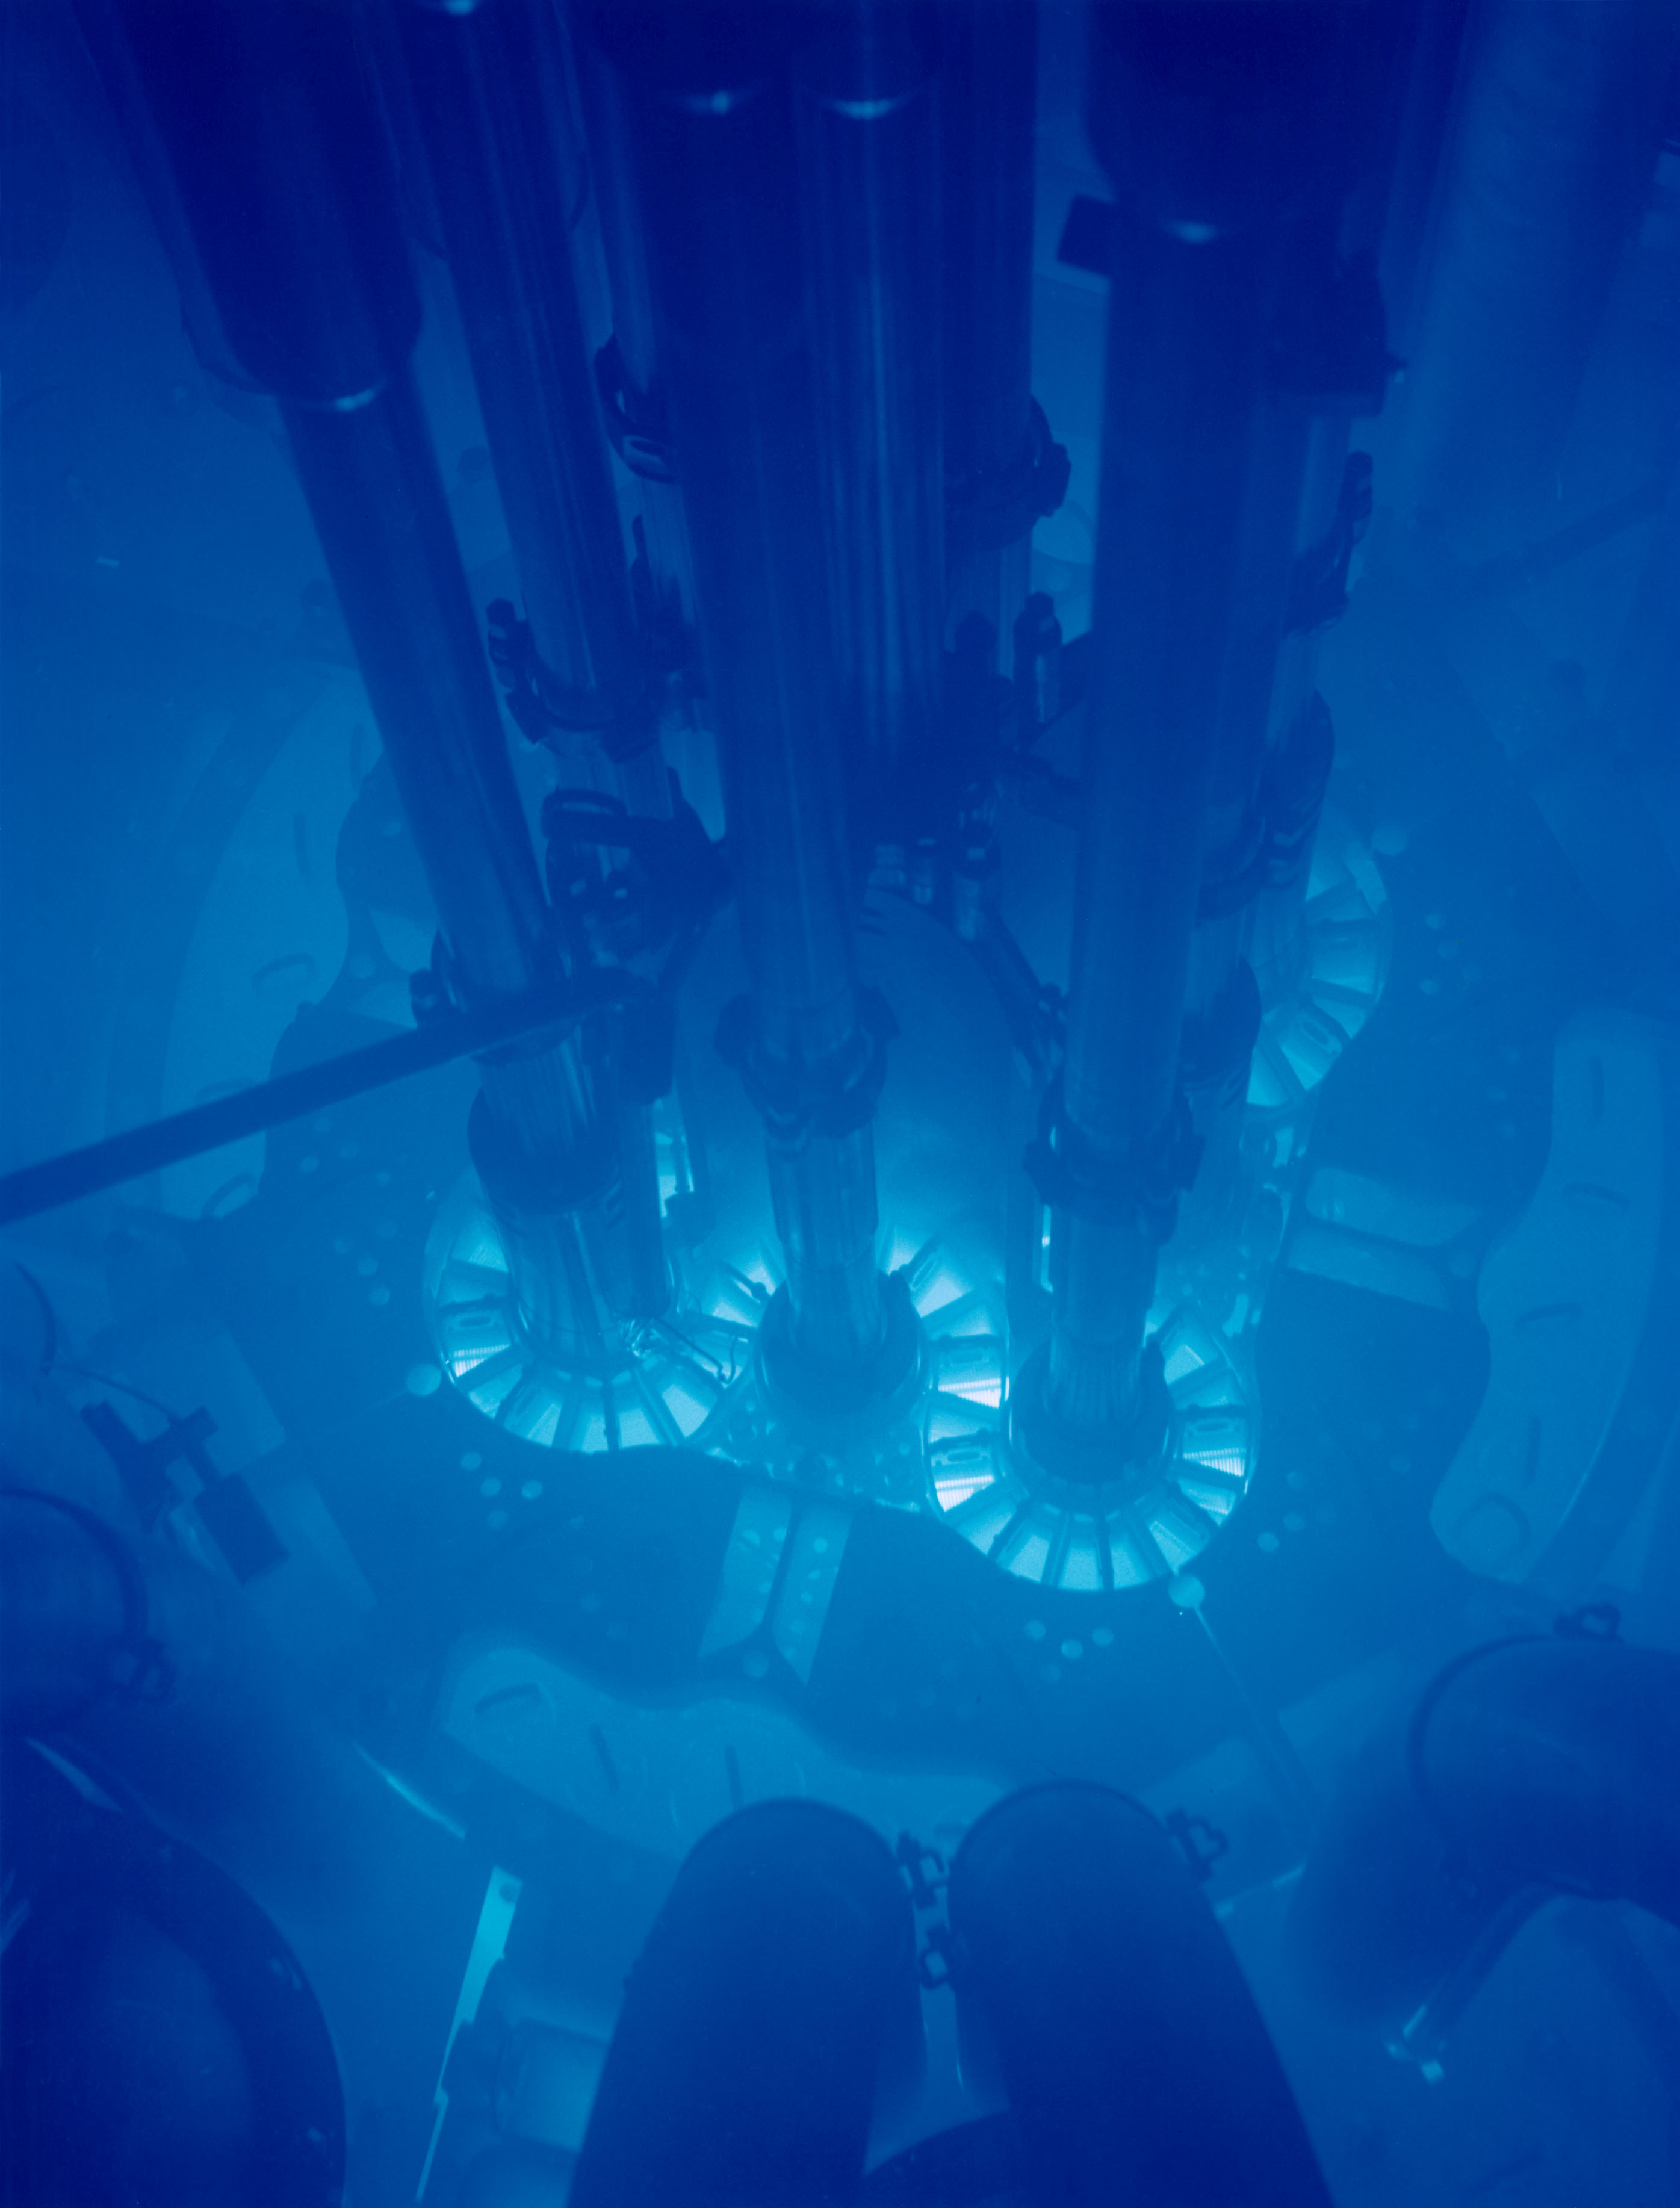
\includegraphics[scale=0.2]{Imagini/Advanced_Test_Reactor.jpg}};
\end{tikzpicture} 
\end{frame}


%frame19
\begin{frame}{\textbf{\underline{Detectorul meu de radiație Cherenkov}}}

\begin{tikzpicture}[overlay, remember picture]
\node[anchor=center, 
      xshift=-3.5cm, 
      yshift=1cm] 
     at (current page.center) 
     {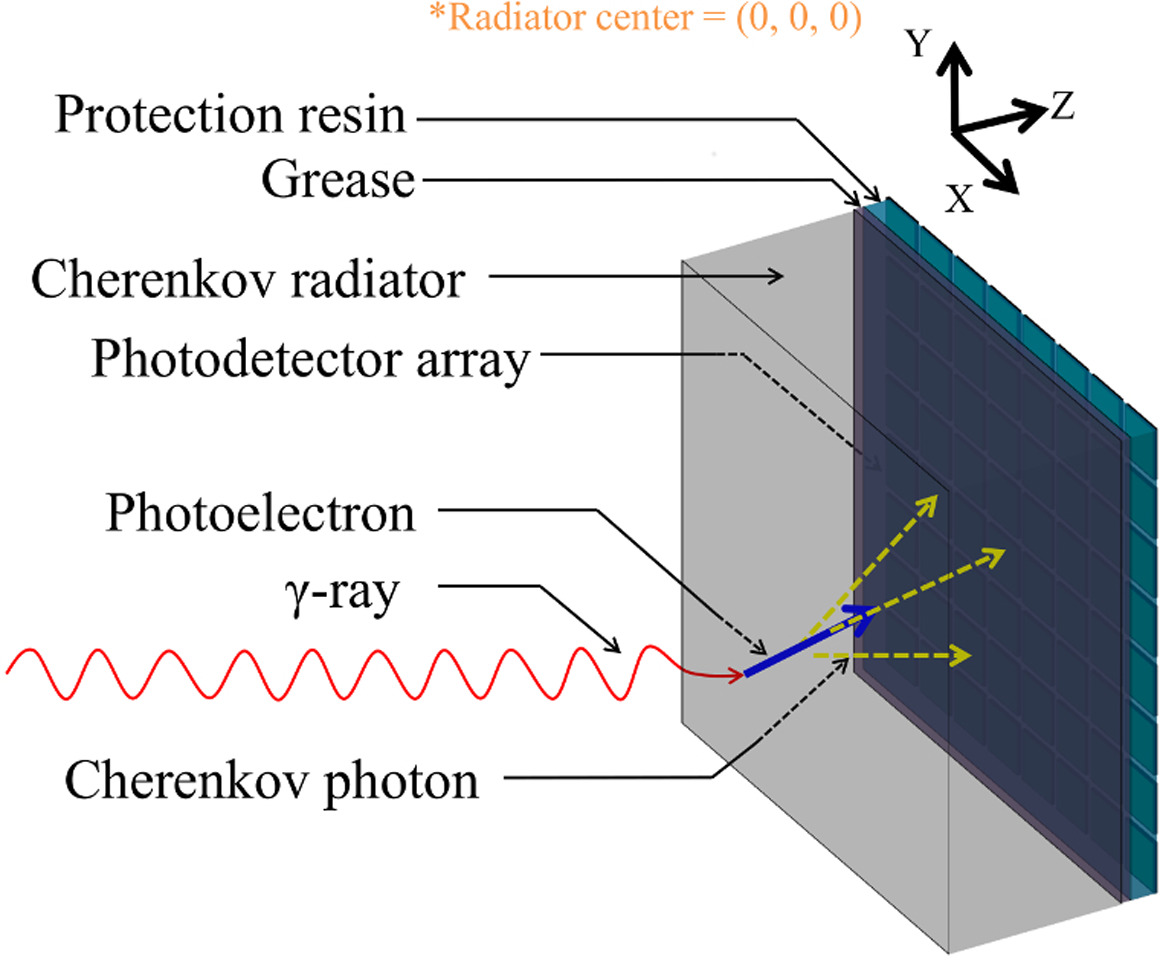
\includegraphics[scale=1]{Imagini/mp12851-fig-0001-m.jpg}};
\end{tikzpicture} 

\begin{tikzpicture}[overlay, remember picture]
\node[anchor=center, 
      xshift=3cm, 
      yshift=1cm] 
     at (current page.center) 
     {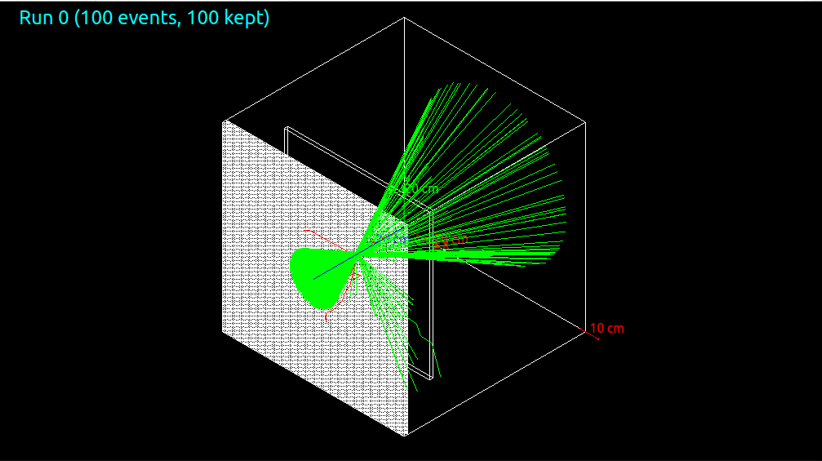
\includegraphics[scale=0.3]{Imagini/Detectorul meu.png}};
\end{tikzpicture} 

\vspace{4cm}
\begin{enumerate}
    \item \makebox[0.5cm]{} O placă din aerogel(transparentă) este străbătută de un proton(albastru) și emite un flux conic de fotoni gamma(verzi).
    \item \makebox[0.5cm]{} Fotoni emiși ajung pe o matrice de 100x100 detectori fotosensibili(voxeli) unde sunt detectați și contabilizați.
\end{enumerate}
\end{frame}


%frame20
\begin{frame}{\textbf{\underline{Output Grafic}}}

\begin{tikzpicture}[overlay, remember picture]
\node[anchor=center, 
      xshift=0cm, 
      yshift=-0.35cm] 
     at (current page.center) 
     {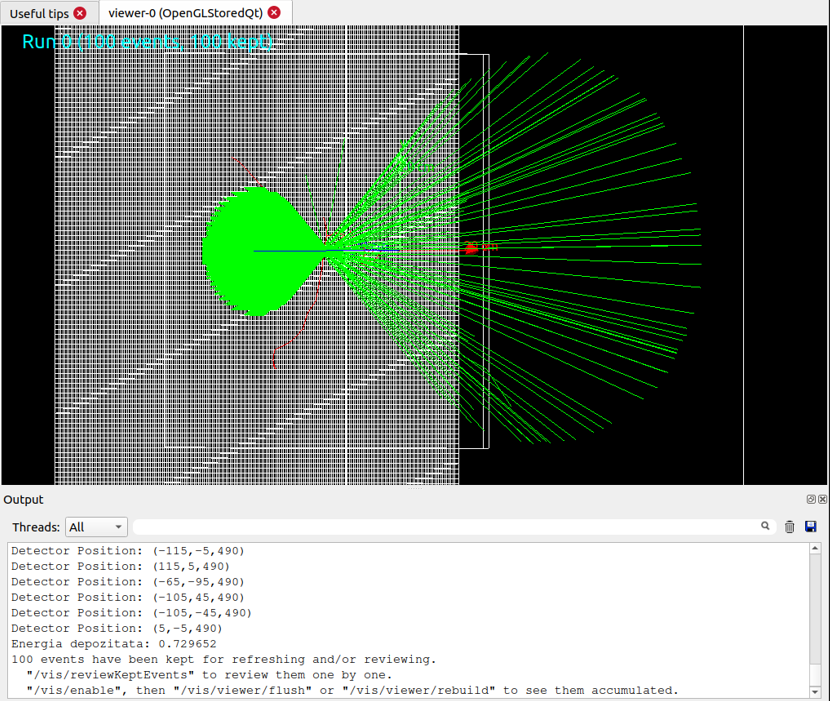
\includegraphics[scale=0.4]{Imagini/DetectorC.png}};
\end{tikzpicture} 

\end{frame}


%frame21
\begin{frame}{}

\begin{tikzpicture}[overlay, remember picture]
\node[anchor=center, 
      xshift=0cm, 
      yshift=0cm] 
     at (current page.center) 
     {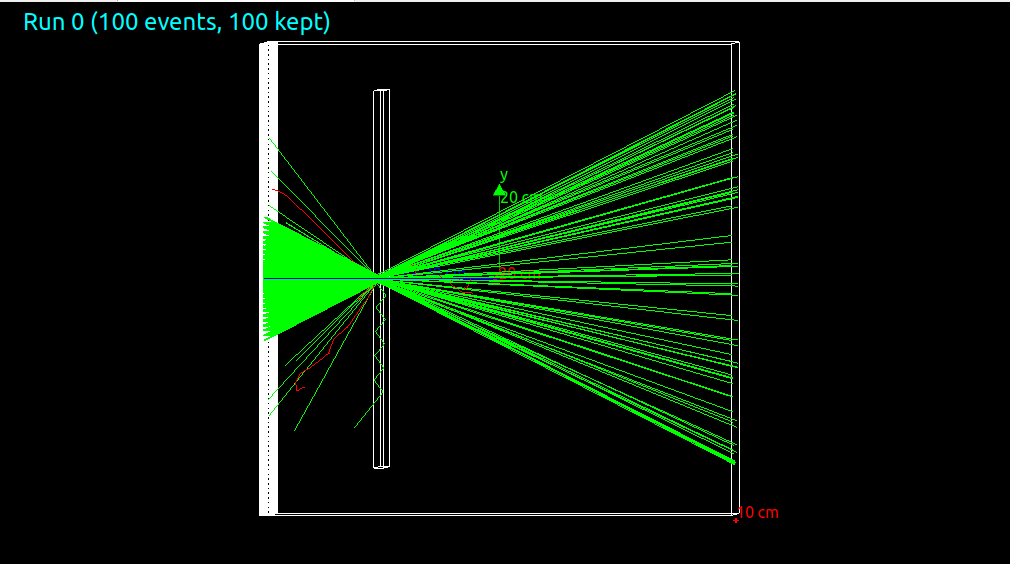
\includegraphics[scale=0.35]{Imagini/Perspective.png}};
\end{tikzpicture} 

\end{frame}


%frame22
\begin{frame}{\textbf{Spectrul radiației Cherenkov - histograma1}}

\begin{tikzpicture}[overlay, remember picture]
\node[anchor=center, 
      xshift=0cm, 
      yshift=0cm] 
     at (current page.center) 
     {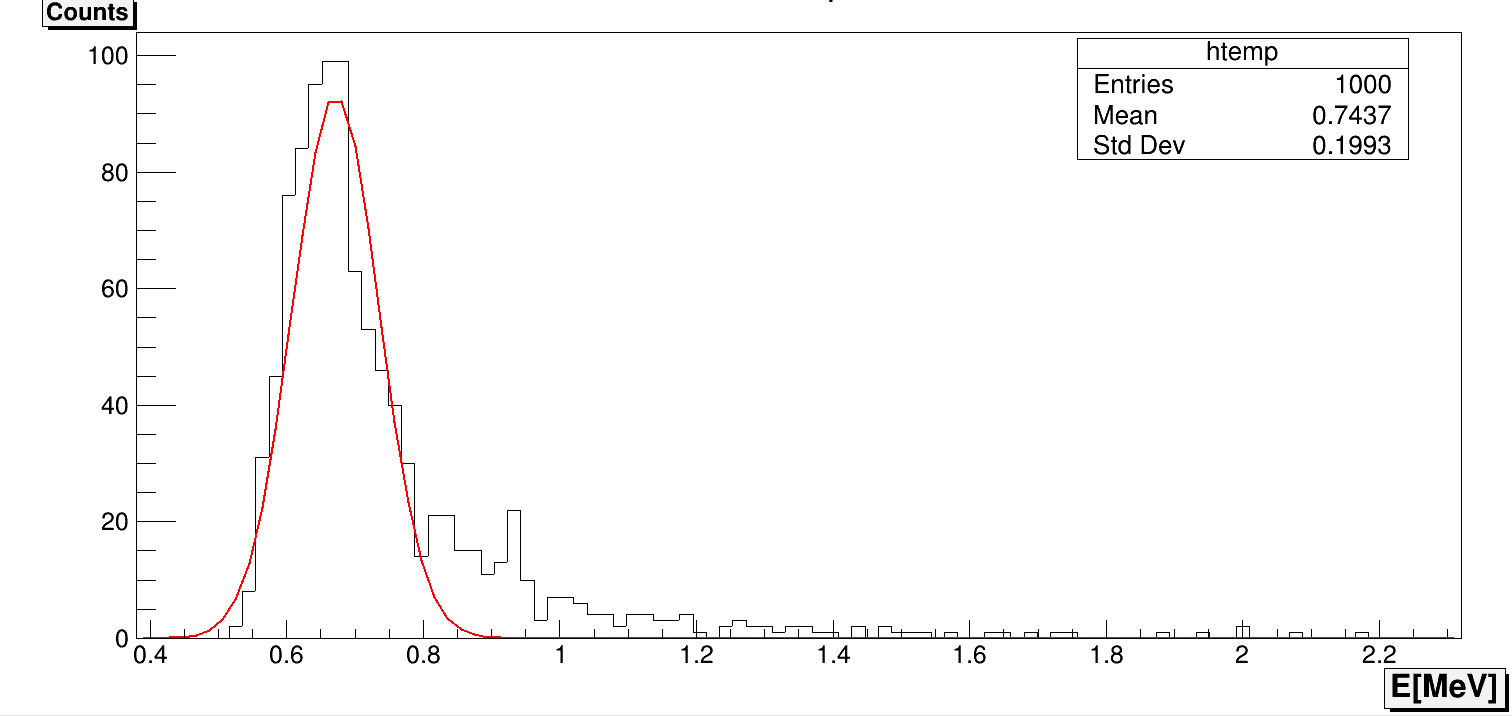
\includegraphics[scale=0.3]{Imagini/SpectrumRadiatieiCherenkov.png}};
\end{tikzpicture} 

\end{frame}


%frame23

\begin{frame}{\textbf{Nr de fotoni funcție de nr de evenimente - histograma2}}

\begin{tikzpicture}[overlay, remember picture]
\node[anchor=center, 
      xshift=0cm, 
      yshift=0cm] 
     at (current page.center) 
     {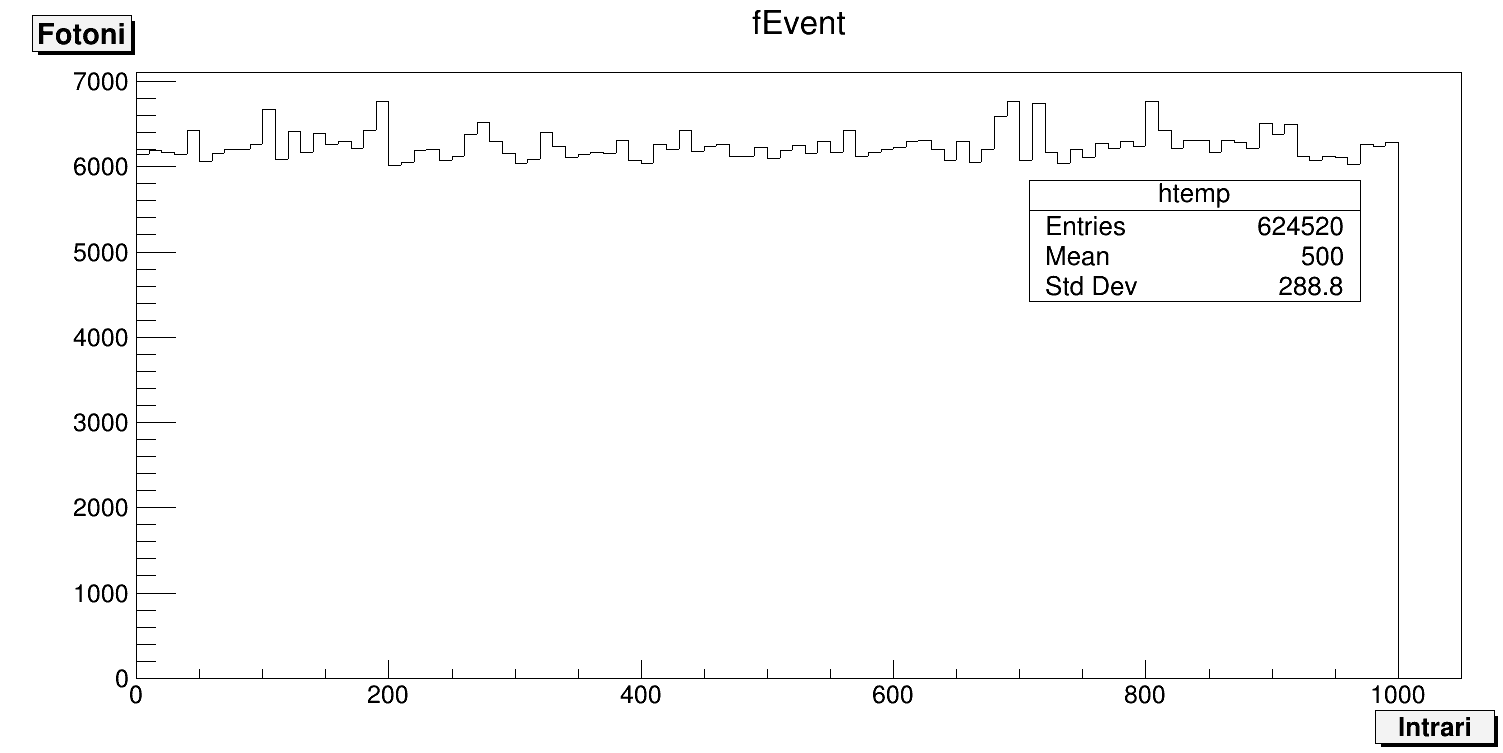
\includegraphics[scale=0.21]{Imagini/Distributia nr de fotoni functie de nr de evnimente.png}};
\end{tikzpicture} 

\end{frame}


%frame24

\begin{frame}{\textbf{Distribuția pe OX a foto-senzorilor - histograma3}}

\begin{tikzpicture}[overlay, remember picture]
\node[anchor=center, 
      xshift=0cm, 
      yshift=0cm] 
     at (current page.center) 
     {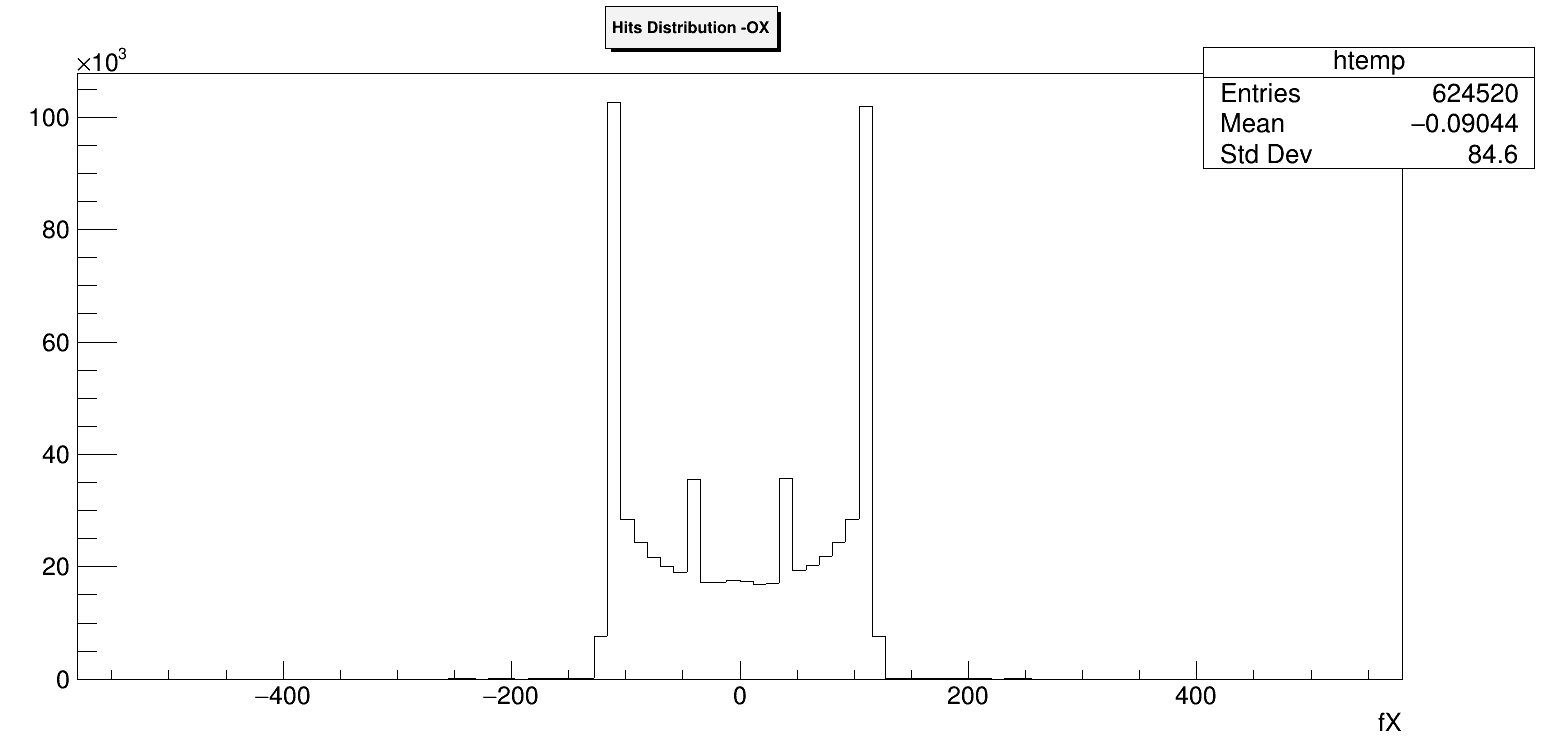
\includegraphics[scale=0.21]{Imagini/Distrib pe Ox a fotosenziorilor.png}};
\end{tikzpicture} 

\end{frame}


%frame25

\begin{frame}{\textbf{Distribuția pe OY a foto-senzorilor - histograma4}}

\begin{tikzpicture}[overlay, remember picture]
\node[anchor=center, 
      xshift=0cm, 
      yshift=0cm] 
     at (current page.center) 
     {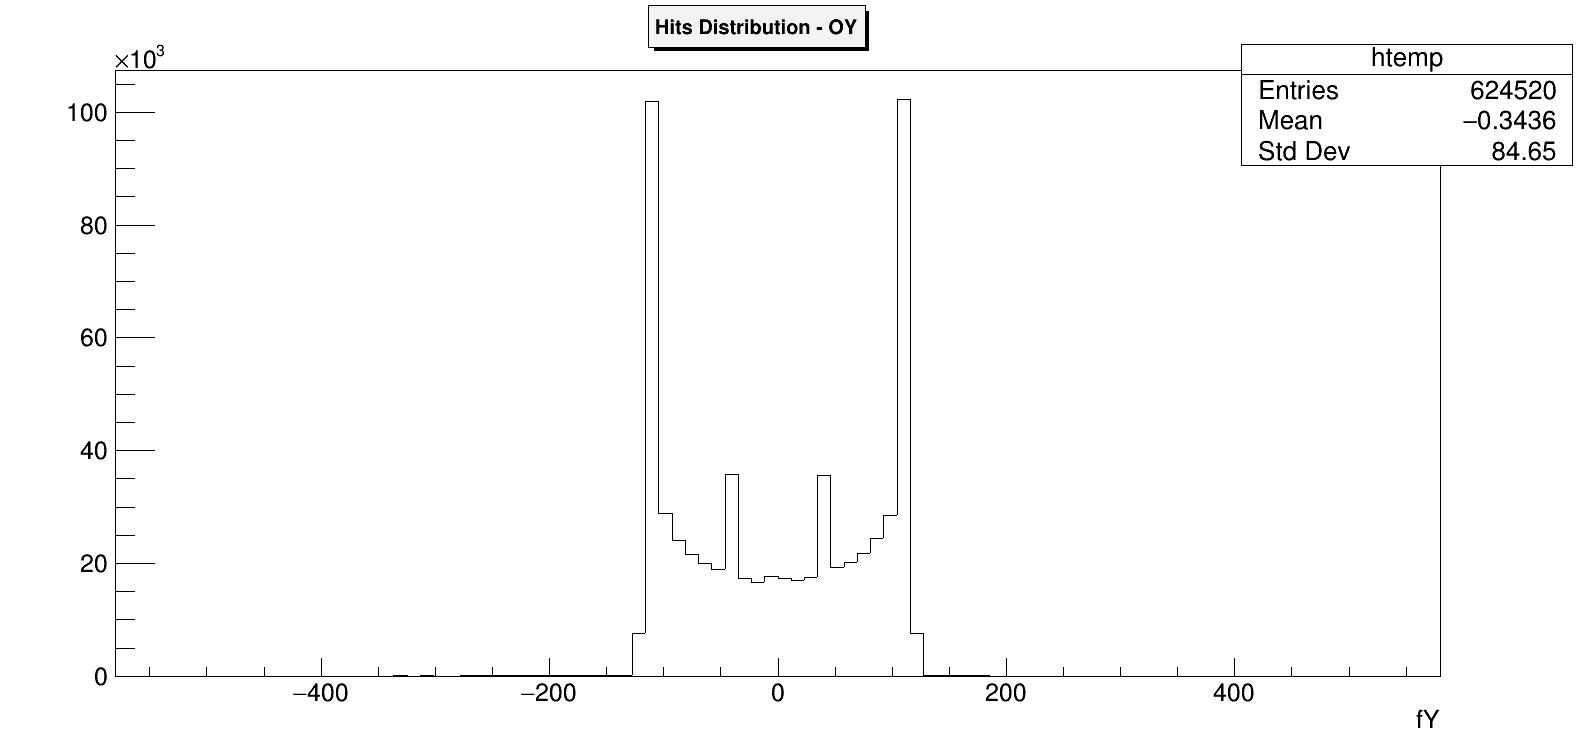
\includegraphics[scale=0.21]{Imagini/Distributia pe Oy a fotosensorilor.png}};
\end{tikzpicture} 

\end{frame}


%frame25

\begin{frame}{\textbf{Corelarea celor două distribuții precedente - color map}}

\begin{tikzpicture}[overlay, remember picture]
\node[anchor=center, 
      xshift=0cm, 
      yshift=0cm] 
     at (current page.center) 
     {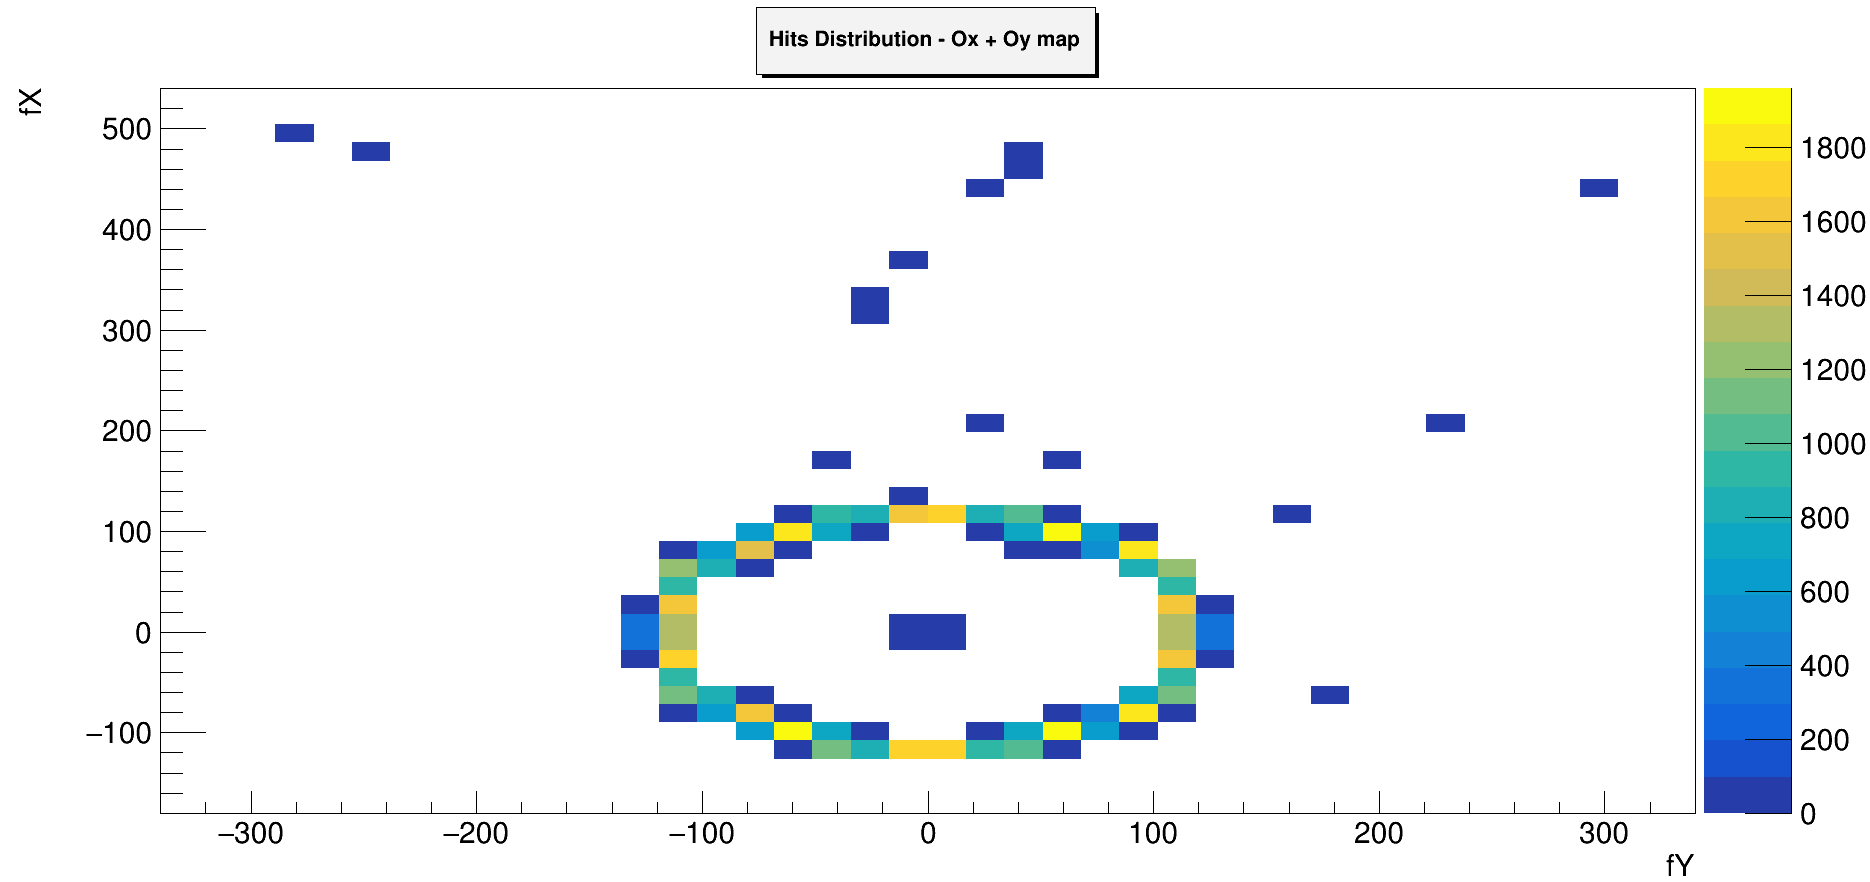
\includegraphics[scale=0.18]{Imagini/RingPattern.png}};
\end{tikzpicture} 

\end{frame}


%frame26

\begin{frame}{\textbf{Ring pattern - din simulare}}

\begin{tikzpicture}[overlay, remember picture]
\node[anchor=center, 
      xshift=0cm, 
      yshift=-0.5cm] 
     at (current page.center) 
     {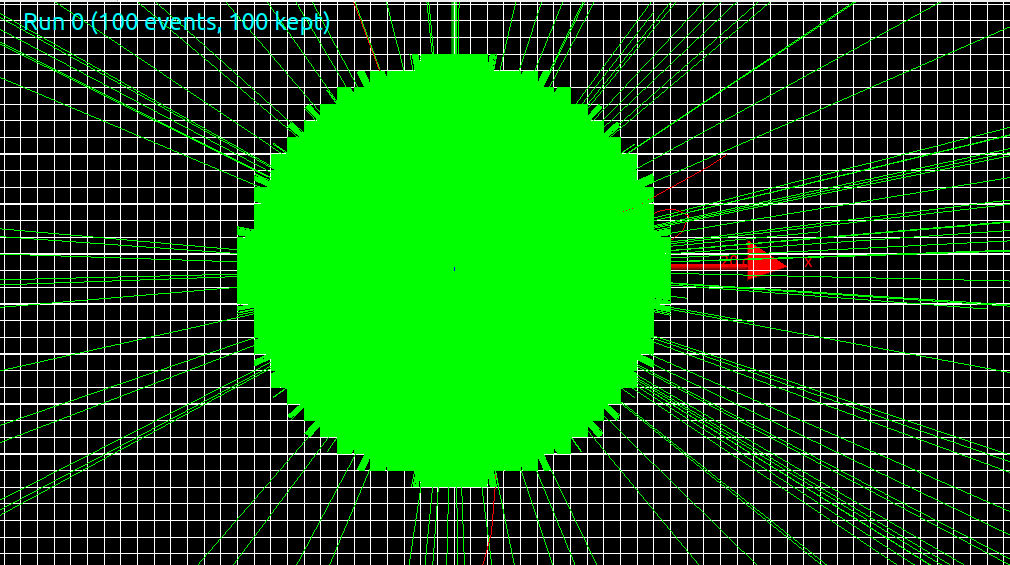
\includegraphics[scale=0.35]{Imagini/RealRing.png}};
\end{tikzpicture} 

\end{frame}


%frame27
\begin{frame}{\textbf{Ce face aplicația}}

\vspace{0cm}
\begin{enumerate}

\large
    \item \makebox[0.5cm]{} \textbf{Reprezintă distribuția numărului de fotoni funcție de energiile lor medii - spectrul radiației Cherenkov.}
    \\---------------------------------------------------------------------------
    \item \makebox[0.5cm]{} \textbf{Distribuția grafică a fotonilor Cherenkov emiși.}
    \\---------------------------------------------------------------------------
    \item \makebox[0.5cm]{} \textbf{Distribuția numărului mediu de fotoni în funcție de numărul de evenimente generate.}
    \\---------------------------------------------------------------------------
    \item \makebox[0.5cm]{} \textbf{Distribuția pozițiilor foto-senzorilor atinși de fotonii Cherenkov - hits distribution + afișarea coordonatelor lor.} 
    \\---------------------------------------------------------------------------
    \item \makebox[0.5cm]{} \textbf{Generarea cât mai multor evenimente și plotarea distribuțiilor lor.} 
    
\end{enumerate}
\end{frame}


\section{ \textbf{Finalul prezentării}}

\begin{frame}{}

\begin{tikzpicture}[overlay, remember picture]
\node[anchor=center, 
      xshift=0cm, 
      yshift=0cm] 
     at (current page.center) 
     {
\includegraphics[scale=0.5]{Imagini/Top.png}};
\end{tikzpicture} 

\end{frame}


\section*{Acknowledgement}  
\begin{frame}
\Large
\textcolor{myNewColorA}{\Huge{\centerline{\textbf{Thank you!}}}}

\begin{tikzpicture}[overlay, remember picture]
\node[anchor=center, 
      xshift=0cm, 
      yshift=-2cm] 
     at (current page.center) 
     {
\includegraphics[scale=0.35]{Imagini/Blue-Technology-technology-logo-design.jpg}};
\end{tikzpicture} 


\end{frame}

\end{document}